\chapter{Theoretical foundations}
\label{chap:theory}

\section{The standard model of particle physics}
\subsection{Introduction}

The standard model (SM) of particle physics is a relativistic quantum field theory (QFT), that encompasses all known fundamental particles of matter and their interactions via the strong nuclear force, weak nuclear force, and the electromagnetic force. Gravity, which is not included in SM theory, is many orders of magnitude weaker than the other forces and therefore can be safely ignored when studying the interactions of SM particles in high energy physics experiments. SM theory was established in the 1970s and has remained essentially unchanged since its formation~\cite{Glashow:1961tr,Weinberg:1967tq,Salam:1968rm}, providing extremely successful high energy physics predictions up to the modern day. Most notably, was the prediction of the Higgs boson~\cite{Englert:1964et,HIGGS1964132,Higgs:1964pj,Guralnik:1964eu,PhysRev.145.1156,PhysRev.155.1554}, which was observed experimentally in 2012 by the ATLAS and CMS Collaborations~\cite{Aad:2012tfa,Chatrchyan:2012xdj,Chatrchyan:2013lba}. Nevertheless, the theory falls short in explaining a number of physical observations, including dark matter~\cite{Aghanim:2018eyx}, neutrino oscillations~\cite{Fukuda:1998mi}, and the hierarchy problem~\cite{PhysRevD.13.974,PhysRevD.20.2619}. To be able to efficiently scrutinise the predictions of the SM in the search for beyond-the-standard model (BSM) physics, it is crucial that the theory is well understood.

This chapter begins by introducing the pillars of SM theory. Section~\ref{sec:sm_particlecontent} summarises the particle content of the SM, including both the fundamental constituents of matter (fermions) and the interaction mediators (bosons). Following this, a pedagogical approach to the construction of the SM is provided, adopting the widely-used Lagrangian formalism throughout. Here, the essential notion of a gauge theory is introduced, in the context of quantum electrodynamics (QED), quantum chromodynamics (QCD), and the unification of the electromagnetic and weak forces into the electroweak (EW) interaction. This leads to a description of spontaneous symmetry breaking in the SM, known as the Higgs-Brout-Englert (HEB) mechanism, which is vital for explaining how particles acquire mass. 

\subsection{Particle content}\label{sec:sm_particlecontent}
In the SM, the fundamental particles of matter and interaction mediators are described as relativistic fields; it is the quantised excitation of these fields which manifest as the physical particles that we observe in nature. The complete particle content of the SM is shown in Figure~\ref{fig:sm_particlecontent}.

\begin{figure}[htb!]
  \centering
  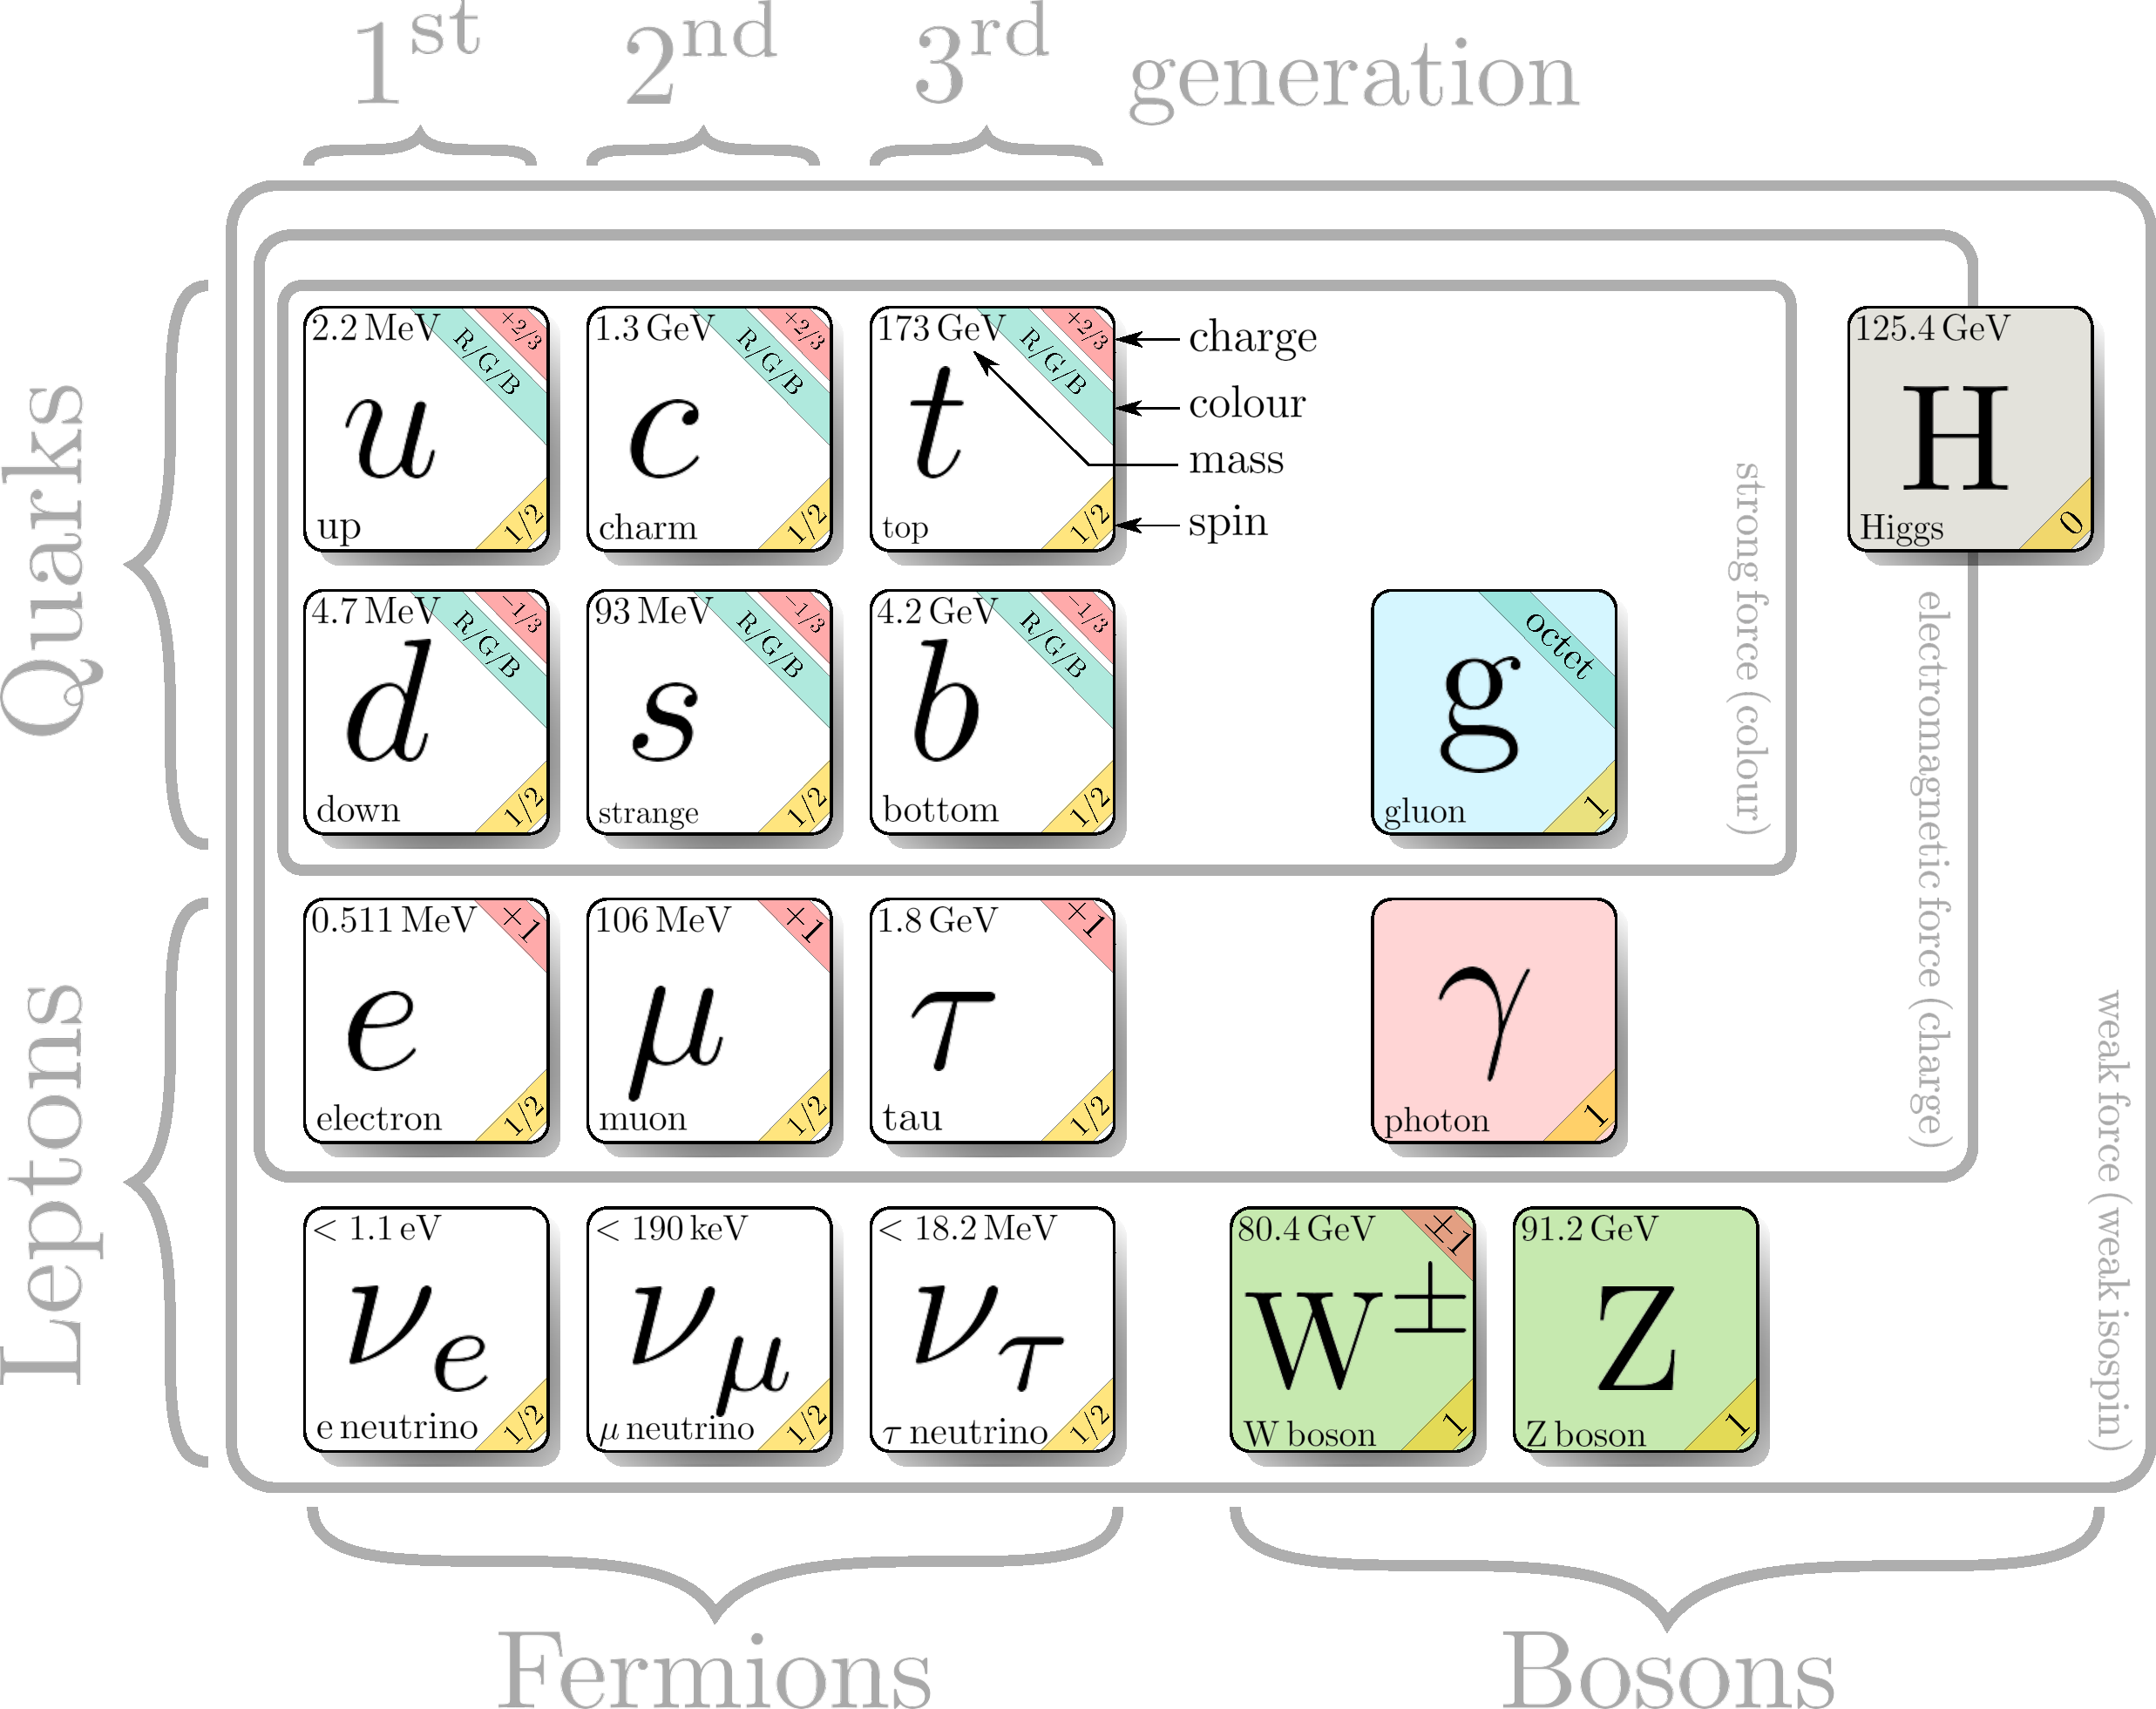
\includegraphics[width=1\linewidth]{Figures/theory/sm_drawing.pdf}
  \caption[Particle content of the SM]
  {
    Particle content of the SM. The charge, colour, and spin quantum numbers are provided for each particle, in addition to their measured masses. All masses are taken from Ref.~\cite{Zyla:2020zbs}, except the Higgs boson (H) mass which is taken from Ref.~\cite{Sirunyan:2020xwk}.
  }
  \label{fig:sm_particlecontent}
\end{figure}

Ignoring the Higgs boson (H) for now, the SM particles can be divided into two groups: the spin-$\frac{1}{2}$ fermions which comprise the matter content of the SM, and the spin-1 gauge bosons which mediate the fundamental interactions. The fermions themselves come in two types: those which interact via the strong force are referred to as \textit{quarks}, whilst those that do not are referred to as \textit{leptons}. The quarks ($q$) are defined in three generations (at different mass scales) and are split into up-type and down-type quarks with charges of $+\frac{2}{3}$ and $-\frac{1}{3}$, respectively (in units of the elementary charge, $e$). Quarks also possess a colour charge, which comes in one of three possible states: R, G and B. It is through this colour charge that the quarks interact with the massless gluon (g) colour octet via the strong interaction.

Likewise, the lepton sector is defined in three mass generations, and is split into the charged leptons ($\ell$) and the neutral leptons (neutrinos, $\nu$). Along with the quarks, the charged leptons interact with the massless photon field, $\gamma$, to define the electromagnetic interaction. All fermions\footnote{There is a slight complexity here concerning the helicity states of the weakly-interacting particles, but this will be addressed in the coming sections.}, including the neutrinos, interact via the weak interaction. This occurs via the exchange of the massive vector bosons: W$^{\pm}$ bosons (charged current interactions) and the Z boson (neutral current interactions). Each fermion in the SM has a corresponding antiparticle, which has the same mass but opposite charge and parity to the respective particle\footnote{In fact, it is not yet known if the neutrino behaves as a Dirac fermion or a Majorana fermion, where the latter describes a fermion that is its own antparticle. This subtle detail is not relevant for this thesis.}.

The final piece in the puzzle is the spin-0 Higgs boson. Electroweak symmetry breaking via the HEB mechanism is essential in the SM as the means in which the W$^{\pm}$ and Z bosons acquire their mass. Additionally, the Yukawa interactions between the quarks/charged leptons and the Higgs field explain the masses of the fermions. The salient feature of the HEB mechanism is the existence of an additional scalar boson: the Higgs boson, the measurements of which form the basis of this thesis.

\subsection{Constructing the Lagrangian}\label{sec:theory_sm}
The SM can be neatly expressed as a Lagrangian density, $\mathcal{L}_{\rm{SM}}$, in terms of the particle fields. We can then infer the dynamics and interactions of the fields by applying the principle of least action to $\mathcal{L}_{\rm{SM}}$ (via the Euler-Lagrange equations). 

At the bedrock of SM theory lies the idea of \textit{symmetry}. N\"{o}ther's theorem~\cite{doi:10.1080_00411457108231446} states that if a particular Lagrangian density is invariant under some transformation, then this implies the existence of an associated conservation law. Such an invariant transformation is referred to as a symmetry of the Lagrangian. By inverting the theorem, we find that for each conserved quantity observed in nature, there must be an associated symmetry of the corresponding Lagrangian. For example, a theory which respects the conservation of energy (momentum) is defined by a Lagrangian which is invariant under a temporal (spatial) translation.

The SM is based on a particular type of QFT, known as a \textit{gauge theory}, where the Lagrangian is invariant under \textit{local gauge transformations}. Such transformations shift the phase of the fundamental fields, where (in contrast to global transformations) the size of the shift can be different for different points in spacetime. 
It is worth stressing that the fundamental fields of a QFT are not observed in nature. Instead, in high energy physics experiments we measure quantities derived from the Lagrangian of the theory, such as cross sections, $\sigma$, and decay rates, $\Gamma$, which are combined under the blanket term of \textit{observables}. Crucially, these observables are independent of the phase of the underlying fields, and therefore $\mathcal{L}_{\rm{SM}}$ must be invariant under local gauge transformations. An important consequence of requiring this symmetry, is the introduction of \textit{gauge boson} fields which act as the mediators of the fundamental interactions. Additionally, N\"{o}ther's theorem tells us that a local gauge symmetry leads to the conservation of a physical charge.

In summary, imposing the invariance of $\mathcal{L}_{\rm{SM}}$ under a local gauge transformation introduces gauge boson fields with certain properties, which interact in certain ways with the fundamental matter fields. The form of these interactions are governed by the \textit{symmetry group} of the gauge transformation. The following sections describe the symmetries of $\mathcal{L}_{\rm{SM}}$ that match what we observe in nature, and how they give rise to the electromagnetic, strong and weak interactions.

\subsubsection{Quantum electrodynamics}
The QFT of electromagnetism is known as quantum electrodynamics (QED)~\cite{Aitchison:2003tq}. It describes charged fermions, photons, and their subsequent interactions. Rather profoundly, all of QED can be derived by requiring the invariance of the QED Lagrangian, $\mathcal{L}_{\rm{QED}} \subset \mathcal{L}_{\rm{SM}}$ under local ${\rm{U}}(1)$ transformations:

\begin{equation}\label{eq:u1_gaugeinvariance}
    {\rm{U}}(1): \mathcal{L}_{\rm{QED}} \mapsto \mathcal{L}'_{\rm{QED}} = \mathcal{L}_{\rm{QED}}.
\end{equation}

The equations of motion for spin-$\frac{1}{2}$ fermion fields, $\psi$, are described by the Dirac equation~\cite{doi:10.1098_rspa.1928.0023}. Therefore, $\mathcal{L}_{\rm{QED}}$ contains a Dirac term of the form,

\begin{equation}
    \mathcal{L}_{\rm{QED}} \supset \mathcal{L}_{\rm{Dirac}} = i\bar{\psi}\slashed{\partial}\psi - m_{\psi}\bar{\psi}\psi,
\end{equation}

\noindent
where we have adopted the slash notation, $\slashed{\partial}=\gamma^\mu\partial_\mu$, such that $i\partial_\mu$ is the position space representation of the 4-momentum, $p_\mu$, and $\gamma^\mu$ are the Dirac gamma matrices that obey the anti-commutation relation $\{\gamma^\mu,\gamma^\nu\}=2\eta^{\mu\nu}\mathbb{1}_4$, where $\eta^{\mu\nu}$ is the Minkowski-space metric: $\eta^{\mu\nu}={\rm{diag}}(1,-1,-1,-1)$. The fermion field, $\psi$, is expressed as a four-component Dirac spinor, where the components are interpreted as the spin-up and spin-down eigenstates of the positive energy (particle) and negative energy (antiparticle) solutions of the Dirac equation. The corresponding adjoint field, $\bar{\psi}$, is defined as $\bar{\psi}=\psi^{\dagger}\gamma^0$, where $\psi^{\dagger}$ is the Hermitian conjugate of $\psi$. Finally, the mass of the fermion, $m_{\psi}$, is described by the mass term, $m_{\psi}\bar{\psi}\psi$.

Under a local ${\rm{U}}(1)$ transformation, the fermion field transforms as,

\begin{equation}
    {\rm{U}}(1): \psi \mapsto \psi' = e^{ig\theta(x)}\psi,
\end{equation}

\noindent
where $g$ is a real number, and $\theta$ is a real-valued function that depends on the spacetime co-ordinate, $x$. Applying the transformation to $\mathcal{L}_{\rm{Dirac}}$,

\begin{equation}\label{eq:u1_dirac}
    {\rm{U}}(1): \mathcal{L}_{\rm{Dirac}} \mapsto \mathcal{L}_{\rm{Dirac}}' = \mathcal{L}_{\rm{Dirac}} - \bar{\psi}g\gamma^\mu(\partial_\mu\theta(x))\psi,
\end{equation}

\noindent
introduces an additional term due to the non-vanishing derivative of $\theta(x)$\footnote{This is not present in global ${\rm{U}}(1)$ transformations where $\partial_\mu\theta=0$.}. To reconcile this with the ${\rm{U}}(1)$ gauge invariance shown in equation~\ref{eq:u1_gaugeinvariance}, it is necessary to add another term to $\mathcal{L}_{\rm{QED}}$,

\begin{equation}\label{eq:qed_interaction}
    \mathcal{L}_{\rm{int}} = -g\bar{\psi}\gamma^{\mu}{\psi}A_\mu,
\end{equation}

\noindent
where $A_\mu$ is a (vector) gauge boson field that transforms under local ${\rm{U}}(1)$ transformations as,

\begin{equation}
    {\rm{U}}(1): A_\mu \mapsto A_\mu' = A_\mu - {\partial_\mu\theta(x)}.
\end{equation}

\noindent
This directly cancels the extra term in equation~\ref{eq:u1_dirac}, establishing the gauge invariance of $\mathcal{L}_{\rm{QED}}$. What we have found is beautiful in its simplicity. By demanding the local ${\rm{U}}(1)$ gauge symmetry of the Dirac Lagrangian, we require the existence of the gauge boson field, $A_\mu$, which is precisely the \textit{photon field}. The additional term in the Lagrangian, $\mathcal{L}_{\rm{int}}$, describes the electromagnetic interaction between charged fermions and photons,
as shown by the Feynman diagram in Figure~\ref{fig:eminteraction}, where the quantity $g=|e|\mathcal{Q}$ is the coupling strength of this interaction, with $e$ being the elementary unit charge and $\mathcal{Q}$ the relative charge of fermion, $\psi$. The conserved quantity in the electromagnetic interaction is the electric charge.

\begin{figure}[htb!]
  \centering
  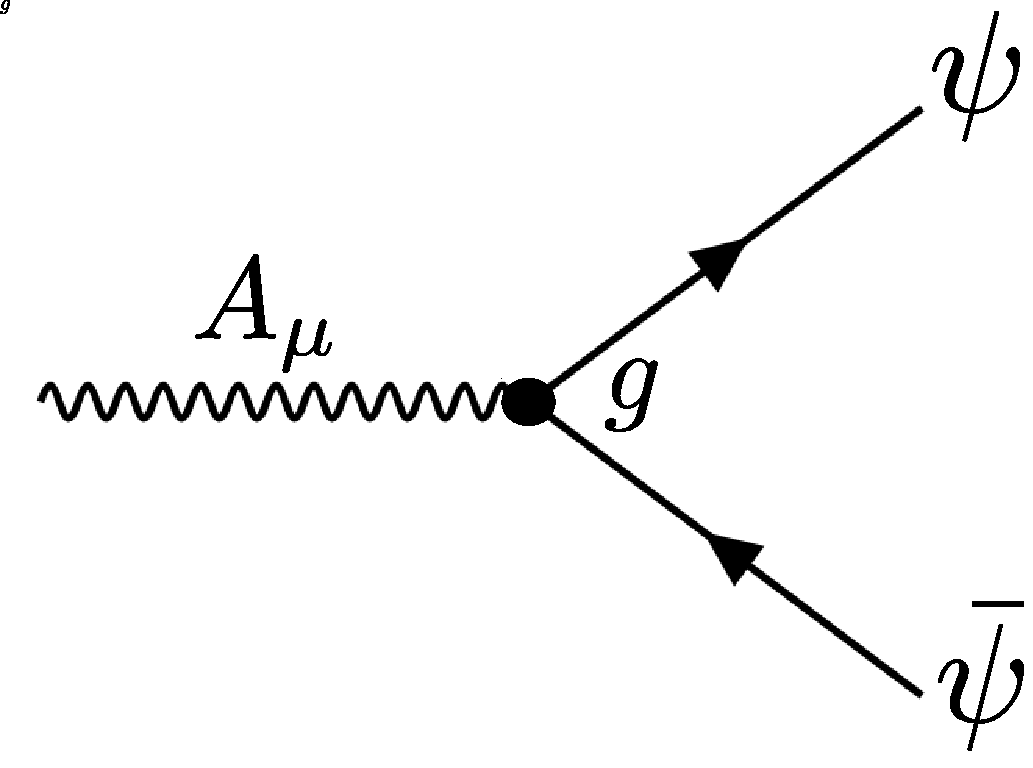
\includegraphics[width=.25\linewidth]{Figures/theory/em_interaction.pdf}
  \caption[The electromagnetic interaction]
  {
    The electromagnetic interaction between the photon field, $A_\mu$, and the charged fermion fields, $\psi$.
  }
  \label{fig:eminteraction}
\end{figure}

The QED Lagrangian is supplemented with the gauge-invariant kinetic term, 

\begin{equation}
    \mathcal{L}_{\rm{QED}} \supset \mathcal{L}_{\rm{gauge}} = -\frac{1}{4}F^{\mu\nu}F_{\mu\nu},
\end{equation}

\noindent
where $F_{\mu\nu}=\partial_{\mu}A_\nu-\partial_{\nu}A_\mu$ is the field strength tensor for the photon field, $A_\mu$. This describes the propagation of the photon field in free space, such that by applying the Euler-Lagrange equations to $\mathcal{L}_{\rm{gauge}}$ we recover Maxwell's equations of electromagnetism~\cite{Aitchison:2003tq}. Hence, the total QED Lagrangian can be written as, 
\begin{equation}
    \mathcal{L}_{\rm{QED}} = -\frac{1}{4}F^{\mu\nu}F_{\mu\nu} + i\bar{\psi}\slashed{D}\psi - m_{\psi}\bar{\psi}\psi,
\end{equation}

\noindent
where we have introduced the \textit{covariant derivative} formalism, $\slashed{D} = \gamma^{\mu}D_\mu = \gamma^{\mu}(\partial_{\mu}+igA_\mu)$, which absorbs the gauge boson field, $A_\mu$, into the definition. Importantly, there is no mass term ($\propto m_A^2 A^{\mu}A_\mu$) present in the Lagrangian for the gauge boson, as terms of this type are not invariant under local gauge transformations. As a consequence, the photon field is massless and the range of the interaction is effectively infinite.

\subsubsection{Extending to {\rm{SU}}(N)}
The strong and weak interactions are obtained by extending the concept of gauge invariance to ${\rm{SU}}({\rm{N}})$ symmetry groups~\cite{Aitchison:2004cs}. In the case of QED, gauge invariance was achieved by defining a covariant derivative containing the corresponding gauge boson field. This simple reformulation extends to all symmetry groups: gauge invariance is realised by introducing the covariant derivative, 

\begin{equation}
    D_\mu = \partial_\mu + i g A^a_\mu {\rm{T}}^a
\end{equation}

\noindent
where $A^a_\mu$ are the gauge boson fields, ${\rm{T}}^a$ are the generators of the group algebra, and $g$ is again the coupling strength of the gauge interaction. In the case of the ${\rm{U}}(1)$ symmetry group, there is a single generator (${\rm{T}}=\mathbb{1}$) which results in a single gauge boson: the photon. For ${\rm{SU}}({\rm{N}})$, the generators ${\rm{T}}^a$ form a basis in the group space of dimension ${\rm{N}}^2-1$ (i.e. $a=1,...,{\rm{N}}^2-1$). Symmetries of this type give rise to ${\rm{N}}^2-1$ gauge bosons.

For a generic covariant derivative, $D_\mu$, the corresponding field strength tensor is,
\begin{equation}
\begin{split}
    \mathbf{F}_{\mu\nu} &= \frac{i}{g}[D_\mu,D_\nu] = \partial_\mu A^a_\nu {\rm{T}}^a - \partial_\nu A^a_\mu {\rm{T}}^a + ig[A^b_\mu {\rm{T}}^b,A^c_\nu {\rm{T}}^c]
    \\
    &= {\rm{T}}^a \Big( \partial_\mu A^a_\nu-\partial_\nu A^a_\mu-gf^{abc}A^b_\mu A^c_\nu \Big) 
    \\
    &= {\rm{T}}^a F^a_{\mu\nu},
\end{split}
\end{equation}

\noindent
where $f^{abc}$ are the structure constants of the symmetry group defined by ${[{\rm{T}}^a,{\rm{T}}^b]=if^{abc}{\rm{T}}^c}$. Abelian groups are defined by the property that the generators of the group algebra commute: $f^{abc}=0\, \forall\, a,b,c$\footnote{The ${\rm{U}}(1)$ group of QED is trivially Abelian, since it is defined by a single generator, ${\rm{T}}=\mathbb{1}$.}. For non-Abelian gauge theories, such as those based on an ${\rm{SU}}({\rm{N}})$ symmetry, the generators in general do not commute. This has dramatic consequences for the physics that the theory describes, as can be seen from the gauge term in the Lagrangian,

\begin{equation}
    \mathcal{L}_{\rm{gauge}} = -\frac{1}{4}F^{a,\mu\nu}F^a_{\mu\nu}.
\end{equation}

\noindent
Unlike in the case of QED, $\mathcal{L}_{\rm{gauge}}$ now contains additional terms representing the self-interactions of the gauge bosons: a term $\propto gf^{abc}(\partial^{\mu} A^{a,\nu})A^b_{\mu}A^c_\nu$ which corresponds to the triple gauge boson interactions, and a term $\propto g^2f^{abc}f^{ade}A^{b,\mu}A^{c,\nu}A^d_{\mu}A^e_\nu$ which corresponds to the quartic gauge boson interactions. These self-interactions are shown as Feynman diagrams in Figure~\ref{fig:gauge_selfinteraction}.

\begin{figure}[htb!]
  \centering
  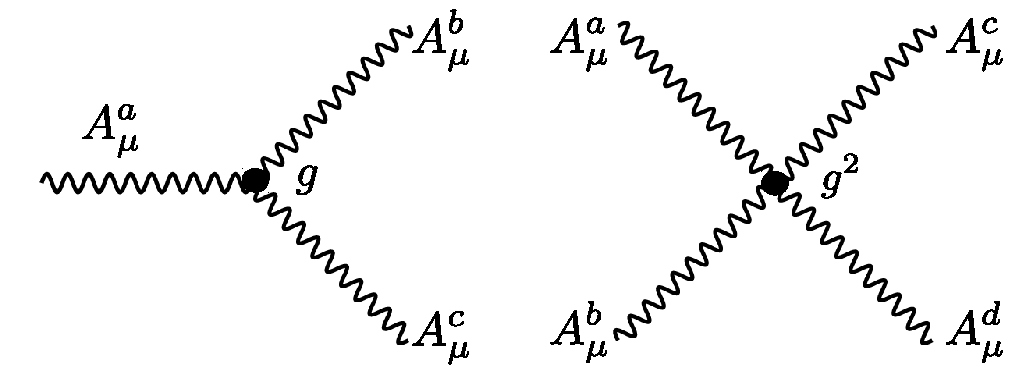
\includegraphics[width=.6\linewidth]{Figures/theory/gauge_self_interaction.pdf}
  \caption[The gauge boson self-interactions]
  {
    The triple (left) and quartic (right) gauge boson self-interactions.
  }
  \label{fig:gauge_selfinteraction}
\end{figure}

\subsubsection{Quantum chromodynamics}
The QFT of the strong interaction, known as quantum chromodynamics (QCD), is established by requiring $\mathcal{L}_{\rm{QCD}} \subset \mathcal{L}_{\rm{SM}}$ to be symmetric under local ${\rm{SU}}(3)_{\rm{C}}$ transformations:

\begin{equation}
    {\rm{SU}}(3)_{\rm{C}}: \mathcal{L}_{\rm{QCD}} \longrightarrow \mathcal{L}'_{\rm{QCD}} = \mathcal{L}_{\rm{QCD}},
\end{equation}

\noindent
where the subscript ${}_{\rm{C}}$ indicates that the transformation only applies to fields with colour charge. The gauge invariance is achieved by replacing $\partial_\mu$ with the covariant derivative, 

\begin{equation}
    D_\mu = \partial_\mu + i g_s G^a_\mu \frac{\lambda^a}{2}.
\end{equation}

\noindent
Here, $\frac{\lambda^a}{2}$ are the $3^2-1=8$ generators of the ${\rm{SU}}(3)_{\rm{C}}$ group algebra, known as the Gell-Mann matrices, and $G^a_\mu$, correspond to the eight gluon fields which mediate the strong interaction. The strength of this interaction is encoded by the coupling strength, $g_s$.

By N\"{o}ther's theorem, we can relate this ${\rm{SU}}(3)_{\rm{C}}$ symmetry to the conservation of colour charge. Quark fields possess a colour charge and therefore interact with the gluon fields. Including the Dirac terms for the quark fields, we arrive at an expression for the QCD Lagrangian,

\begin{equation}
    \mathcal{L}_{\rm{QCD}} = \sum_j i\bar{\psi}_j(\slashed{D}-m_j)\psi_j - \frac{1}{4} G^{a,\mu\nu}G^a_{\mu\nu}.
\end{equation}

\noindent
where $\psi_j$ are the quark spinors of flavour $j=\{u,d,c,s,t,b\}$. As described in the previous section, the non-commutative properties of the Gell-Mann matrices lead to the gluon self-interactions~\cite{Halzen:1984mc}. These self-interactions have major consequences for the physics of the strong interaction. Firstly, the coupling strength, $g_s$, decreases as a function of the interaction energy scale\footnote{This property is related to the $\beta$-function of QCD; a discussion of which is left to Ref.~\cite{Halzen:1984mc}.}. At very high energies, such as those probed in the hard scatterings at the LHC, the strong force is sufficiently weak to describe the quarks and gluons as independent particles using perturbation theory. This effect is referred to as \textit{asymptotic freedom}~\cite{PhysRevLett.30.1343}. On the other hand, at lower energies quarks and gluons are never observed as isolated colour charged particles, but are instead \textit{confined} to colourless bound states, known as hadrons. This gives rise to the plethora of meson ($q\bar{q}$) and baryon/anti-baryon ($qqq/\bar{q}\bar{q}\bar{q}$) states that we observe in nature, and explains why outgoing quarks and gluons in high energy collisions form collimated sprays of hadrons, known as jets~\cite{Salam:2009jx}.

\subsubsection{Electroweak unification}
One of the great successes of SM theory is the unification of the electromagnetic and weak interactions~\cite{Glashow:1961tr,Weinberg:1967tq,Salam:1968rm}. This was achieved by requiring the electroweak Lagrangian, $\mathcal{L}_{\rm{EW}} \subset \mathcal{L}_{\rm{SM}}$ to be symmetric under local ${\rm{SU}(2)_{\rm{L}}}\otimes{\rm{U}}(1)_{\rm{Y}}$ transformations,

\begin{equation}
    {\rm{SU}}(2)_{\rm{L}}\otimes{\rm{U}}(1)_{\rm{Y}}: \mathcal{L}_{\rm{EW}} \longrightarrow \mathcal{L}'_{\rm{EW}} = \mathcal{L}_{\rm{EW}},
\end{equation}

\noindent
which requires the introduction of the covariant derivative,

\begin{equation}\label{eq:ew_covariant}
    D_\mu = \partial_\mu + i g W^i_\mu \frac{\sigma^i}{2} + i g' B_\mu {\rm{Y}}. %\frac{\mathbb{1}}{2} .
\end{equation}

\noindent
The non-Abelian ${\rm{SU}}(2)_{\rm{L}}$ symmetry group has $2^2-1=3$ generators, ${\rm{T}}^i=\frac{\sigma^i}{2}$, which are the $2\times2$ Pauli-spin matrices, with three associated gauge boson fields, $W^i_\mu$. The quantity $g$ represents the coupling strength of this interaction, whilst the corresponding conserved charge is known as weak isospin, $t_3$. The Abelian ${\rm{U}}(1)_{\rm{Y}}$ symmetry has a single generator, ${\rm{T}}={\rm{Y}}=\frac{y}{2}\mathbb{1}$, with a single gauge boson field, $B_\mu$. This interaction has a coupling strength, $g'$, and conserves a quantity referred to as weak hypercharge, $y$. We extract the physical states of the gauge fields (${\rm{W}}^\pm$ bosons, ${\rm{Z}}$ boson and the photon) according to the following relations,

\begin{equation}\label{eq:ew_rotation}
\begin{split}
    W^{\pm}_\mu &= \frac{1}{\sqrt{2}}(W_\mu^1 \mp iW_\mu^2) \\
    \begin{pmatrix}
    Z_\mu \\
    A_\mu
    \end{pmatrix} 
    &= 
    \begin{pmatrix}
    \cos{\theta_W} & -\sin{\theta_W} \\
    \sin{\theta_W} & \cos{\theta_W}
    \end{pmatrix} 
    \begin{pmatrix}
    W^3_\mu \\
    B_\mu
    \end{pmatrix}
\end{split}
\end{equation}

\noindent
where $\theta_W=\tan^{-1}(g'/g)$ is the weak mixing angle, and is measured directly in experiment. The gauge term of the electroweak (EW) Lagrangian,

\begin{equation}
    \mathcal{L}_{\rm{EW}} \supset \mathcal{L}_{\rm{gauge}} = -\frac{1}{4}W^{i,\mu\nu}W^i_{\mu\nu} - \frac{1}{4}B^{\mu\nu}B_{\mu\nu},
\end{equation}

\noindent
introduces self-interactions between the $W^i_\mu$ fields, which after rotating to the physical states are observed as the $\gamma\rm{W^+W^-}$ and ${\rm{Z W^+W^-}}$ triple gauge interactions, and the $\rm{W^+W^-W^+W^-}$, $\rm{W^+W^-ZZ}$ and ${\rm{W^+W^-}}\gamma\gamma$ quartic gauge interactions.

Turning our attention to the fermions, the diagram in Figure~\ref{fig:sm_particlecontent} tells us that both quarks and leptons interact via the weak interaction. In nature, we observe the weak interaction to violate parity conservation~\cite{PhysRev.105.1413}, or in other words, the weak interaction behaves differently under the spatial translation: $x\mapsto-x$. A fermion field, $\psi$, can be projected into its left-handed and right-handed components, $\psi_L$ and $\psi_R$, using the projection operators, $\hat{P}_{L/R} = \frac{1}{2}(1\mp\gamma^5)$, where $\gamma^5=\gamma^0\gamma^1\gamma^2\gamma^3$. We can then bake the effect of parity violation into EW theory by only permitting interactions between the $W^i_\mu$ gauge fields and left-handed fermions\footnote{Hence the use of the subscript, ${}_{\rm{L}}$, in the ${\rm{SU}}(2)$ symmetry group definition.} (right-handed anti-fermions)~\cite{Aitchison:2004cs}. In this way, the left-handed components of the fermion fields transform as doublets under ${\rm{SU}}(2)_{\rm{L}}$ transformations ($t_3=\pm\frac{1}{2}$), whilst the right-handed components transform as singlets ($t_3=0$),

\begin{equation}
\begin{split}
    \psi_L&: \quad L_{jL} = \begin{pmatrix}
    \nu_{jL} \\
    \ell_{jL}
    \end{pmatrix}, \quad Q^a_{jL} = \begin{pmatrix}
    u^a_{jL} \\
    d^a_{jL}
    \end{pmatrix},
    \\
    \psi_R&: \quad \ell_{jR}, \quad u^a_{jR}, \quad d^a_{jR}.
\end{split}
\end{equation}

\noindent
Here, $\ell$ and $\nu$ represent the charged leptons and neutrinos, $u$ and $d$ represent the up-type and down-type quarks, and the flavour indices, $j$, and colour indices, $a$, are explicitly kept in the notation for completeness. It is important to note that there is no right-handed neutrino field in the standard EW theory, as they do not interact via either the weak or electromagnetic interactions.

The fermionic EW interactions are defined by the following gauge-invariant terms in the Lagrangian,

\begin{equation}\label{eq:ew_interactionterms}
    \mathcal{L}_{\rm{EW}} \supset \bar{\psi}_L i \slashed{D}^L \psi_L + \bar{\psi}_R i \slashed{D}^R \psi_R,
\end{equation}

\noindent
where,

\begin{equation}
\begin{split}
    D^L_\mu &= \partial_\mu \mathbb{1}_2 + igW^i_\mu \frac{\sigma^i}{2} + ig'B_\mu \frac{y_L}{2} \mathbb{1}_2 
    \\
    &= \begin{pmatrix}
    \partial_\mu & 0 \\
    0 & \partial_\mu
    \end{pmatrix} + \frac{ig}{2}\begin{pmatrix}
    W^3_\mu & W^1_\mu-iW^2_\mu \\
    W^1_\mu+iW^2_\mu & -W^3_\mu
    \end{pmatrix} + \frac{ig'y_L}{2}\begin{pmatrix}
    B_\mu & 0 \\
    0 & B_\mu
    \end{pmatrix},
    \\
    D^R_\mu &= \partial_\mu + ig'B_\mu \frac{y_R}{2}
\end{split}
\end{equation}

\noindent
Considering the diagonal elements of $D^L_\mu$ together with $D^R_\mu$, and applying the rotation to the physical basis (equation~\ref{eq:ew_rotation}), we find photon-fermion interaction term ($\bar{\psi}\psi A_\mu$) of the form,

\begin{equation}
\begin{split}
    \mathcal{L}_{\rm{EW}} \supset &-\Big[ \bar{\psi}_L \gamma^\mu(g\sin{\theta_W} \frac{\sigma^3}{2} + g'\cos{\theta_W} \frac{y_L}{2} \mathbb{1}_2)\psi_L \; + \; \bar{\psi}_R\gamma^\mu g'\cos{\theta_W}\frac{y_R}{2}\psi_R \Big]A_\mu,
    \\
    = &-|e|\Big[ \bar{\psi}_L \gamma^\mu (\frac{\sigma^3}{2}+\frac{y_L}{2} \mathbb{1}_2)\psi_L + \bar{\psi}_R\gamma^\mu \frac{y_R}{2}\psi_R \Big]A_\mu,
    \\
    = & - |e|\mathcal{Q} \bar{\psi} \gamma^\mu \psi A_\mu,
\end{split}
\end{equation}

\noindent
where the relations, $g\sin{\theta_W}=|e|$ and $g'\cos{\theta_W}=|e|$, are inferred by relating to the equivalent interaction term of QED in equation~\ref{eq:qed_interaction}. Moreover, the observation that the electromagnetic interaction does not depend on the handedness (chirality state) of the fermion field tell us,

\begin{equation}\label{eq:ew_unification}
    \mathcal{Q} = t_3 + \frac{y}{2}.
\end{equation}

\noindent
This is ultimately the defining relation of electroweak unification. At first glance, the electromagnetic and weak interactions appear to have completely different properties. The electromagnetic interaction is parity-conserving and is mediated by the massless photon over an effectively infinite range, whilst the weak interaction is parity-violating, and is mediated by the massive weak bosons, over a very short interaction range. Nevertheless, this section has proved that the two can be unified into a common electroweak theory, where equation~\ref{eq:ew_unification} tells us how the charge of the electromagnetic interaction is related to the weak isospin and hypercharge. Using this relation, the full set of electroweak quantum numbers for the SM fields are derived to be the values shown in Table~\ref{tab:ew_quantumnumbers}. Following the same procedure as shown for the $\bar{\psi}\psi A_\mu$ interaction, the charged current (${\rm{W}}^{\pm}$) and neutral current (${\rm{Z}}$) weak interactions are derived from the Lagrangian in equation~\ref{eq:ew_interactionterms}, providing the full set of fermionic EW interactions displayed in Figure~\ref{fig:feynman_ew}.

\begin{figure}[htb!]
  \centering
  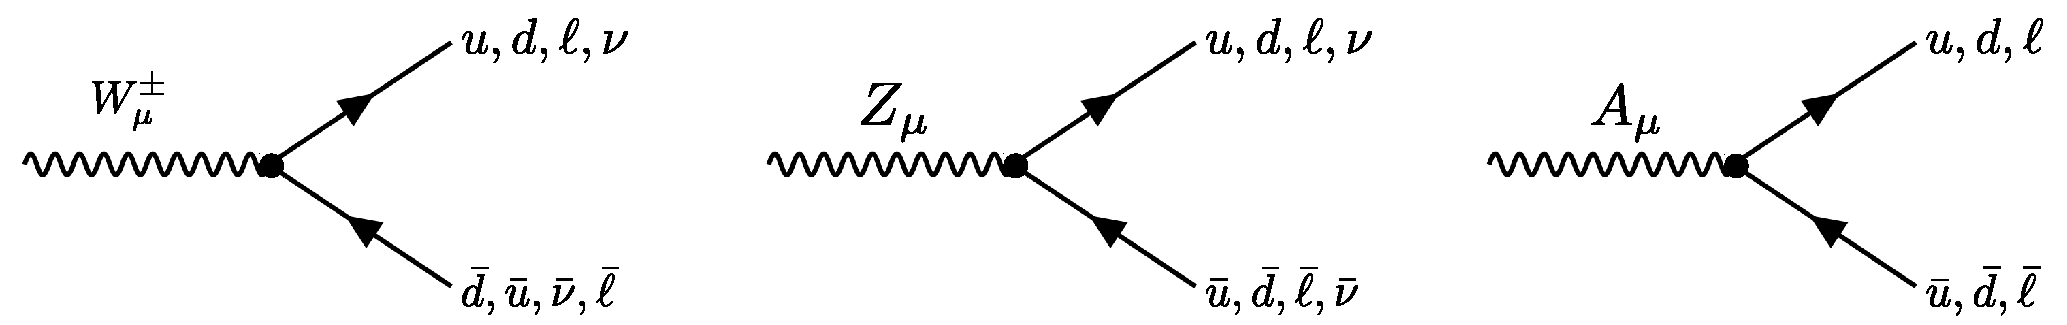
\includegraphics[width=.9\linewidth]{Figures/theory/ew_interaction.pdf}
  \caption[The electroweak interaction including fermions]
  {
    The electroweak interactions including fermions.
  }
  \label{fig:feynman_ew}
\end{figure}

\begin{table}[htb!]
    \caption[The electroweak quantum numbers of the SM fields]{The weak isospin ($t_3$), weak hypercharge ($y$) and electric charge ($\mathcal{Q}$) quantum numbers of the standard model fields. Here, the fermion flavour states are explicitly shown.}
    \label{tab:ew_quantumnumbers}
    % \vspace{.5cm}
    \centering
    % \scriptsize
    \renewcommand{\arraystretch}{1.2}
    \setlength{\tabcolsep}{20pt}
    % \hspace*{-1.5cm}
    \begin{tabular}{l|ccc}
   Particle field & $t_3$ & $y$ & $\mathcal{Q}=t_3+\frac{y}{2}$ \\ \hline
   $u^a_L$, $c^a_L$, $t^a_L$ & $+\frac{1}{2}$ & $+\frac{1}{3}$ & $+\frac{2}{3}$ \\
   $d^a_L$, $s^a_L$, $b^a_L$ & $-\frac{1}{2}$ & $+\frac{1}{3}$ & $-\frac{1}{3}$ \\
   $u^a_R$, $c^a_R$, $t^a_R$ & $0$ & $+\frac{4}{3}$ & $+\frac{2}{3}$ \\
   $d^a_R$, $s^a_R$, $b^a_R$ & $0$ & $-\frac{2}{3}$ & $-\frac{1}{3}$ \\
   \hline
   $\nu_{eL}$, $\nu_{{\mu}L}$, $\nu_{{\tau}L}$ & $+\frac{1}{2}$ & $-1$ & $0$ \\
   $e_L$, $\mu_L$, $\tau_L$ & $-\frac{1}{2}$ & $-1$ & $-1$ \\
   $e_R$, $\mu_L$, $\tau_L$ & $0$ & $-2$ & $-1$ \\
   \hline
   $W^{\pm}_\mu$ & $\pm 1$ & $0$ & $\pm 1$ \\
   $Z_\mu$ & $0$ & $0$ & $0$ \\
   $A_\mu$ & $0$ & $0$ & $0$ \\
   $G^a_{\mu}$ & $0$ & $0$ & $0$ \\
   \hline
   $H$ & $-\frac{1}{2}$ & $1$ & $0$
\end{tabular}
    % \hspace*{-1.5cm}
\end{table}

% \begin{equation}
% \begin{split}
%     \mathcal{L}_{\rm{EW}} \supset {} &-\frac{g}{\sqrt{2}}W^+_\mu \bar{u}_L \gamma^\mu d_L - \frac{g}{\sqrt{2}}W^+_\mu \bar{\nu}_L \gamma^\mu \ell_L + {\rm{h.c.}}
%     \\
%     &-\frac{g}{\cos{\theta_W}}Z_\mu \psi \gamma^\mu (\frac{\sigma^3}{2}\hat{P}_L - \sin{\theta_W}^2\mathcal{Q})\psi
% \end{split}
% \end{equation}

% \noindent
% Clearly, the $W^{\pm}$ boson terms (charged current) describe the interactions between up-type and down-type quarks and between charged leptons and neutrinos, whilst the $Z$ boson terms (neutral current) describe the interactions between fermions of the same type. All fermionic EW interactions are shown by the Feynman diagrams in Figure~\ref{fig:feynman_ew}.

\FloatBarrier
\subsubsection{Spontaneous symmetry breaking}
By simply applying the elegant principle of gauge invariance, we have constructed a Lagrangian density that describes all of the fundamental interactions between the fermions and the vector gauge bosons, as well as the gauge boson self interactions of the strong and weak forces. Nevertheless, there is a striking omission: a consistent description of the \textit{particle masses}. As in QED, gauge boson mass terms of the form $\propto m_W^2W^{i,\mu}W^i_\mu$ are forbidden in electroweak theory as they are not invariant under local ${\rm{SU}(2)_{\rm{L}}}\otimes{\rm{U}}(1)_{\rm{Y}}$ transformations. This contradicts the masses of the ${\rm{W}}^{\pm}$ and Z bosons observed in experiment. Moreover, mass terms for the fermion fields, $\propto m_{\psi}(\bar{\psi}_L\psi_R+\bar{\psi}_R\psi_L)$ are also not gauge invariant due to the different transformation properties of the left-handed and right-handed fields. In SM theory, we introduce the Higgs-Brout-Englert (HEB) mechanism~\cite{Englert:1964et,HIGGS1964132,Higgs:1964pj,Guralnik:1964eu,PhysRev.145.1156,PhysRev.155.1554} to generate the particle masses by spontaneously breaking the symmetry of the electroweak interaction.

A spontaneous symmetry breaking (SSB) refers to the case where the underlying Lagrangian of the theory obeys certain symmetries, whereas the lowest energy (vacuum) state of the corresponding Hamiltonian does not~\cite{Aitchison:2004cs}. The HEB mechanism explains what happens when the broken symmetry is a local gauge symmetry. In the SM, the HEB mechanism breaks the ${\rm{SU}(2)_{\rm{L}}}\otimes{\rm{U}}(1)_{\rm{Y}}$ symmetry of the electroweak interaction into a ${\rm{U}}(1)_{\rm{EM}}$ symmetry, as shown in equation~\ref{eq:ssb},

\begin{equation}\label{eq:ssb}
    {\rm{SU}}(3)_{\rm{C}} \otimes {\rm{SU}}(2)_{\rm{L}} \otimes {\rm{U}}(1)_{\rm{Y}} \quad \overset{{\rm{HEB}}}{\mapsto} \quad {\rm{SU}}(3)_{\rm{C}} \otimes {\rm{U}}(1)_{\rm{EM}}.
\end{equation}

\noindent
Note, the ${\rm{SU}}(3)_{\rm{C}}$ symmetry of the strong interaction remains unbroken and therefore the gluon fields, $G^a_{\mu}$, are unaffected. The SSB is achieved via the introduction of two complex scalar fields\footnote{Because the HEB mechanism is required to generate the masses of the weak gauge bosons, one of the complex scalar fields must be neutral, $\phi^0$, whilst the other must be charged, $\phi^+$, such that $(\phi^+)^*=\phi^-$~\cite{Thomson:2013zua}.}, $\phi^+$ and $\phi^0$, which transforms as a doublet, $H$, under ${\rm{SU}}(2)_{\rm{L}}$ transformations,

\begin{equation}
    H = \begin{pmatrix}
    \phi^+ \\
    \phi^0
    \end{pmatrix} = 
    \frac{1}{\sqrt{2}}\begin{pmatrix}
    \phi_1+i\phi_2 \\
    \phi_3+i\phi_4
    \end{pmatrix}.
\end{equation}

\noindent
The doublet, $H$, is referred to as the Higgs field. In total, this corresponds to adding four additional degrees of freedom into the Lagrangian via the ${\rm{SU}(2)_{\rm{L}}}\otimes{\rm{U}}(1)_{\rm{Y}}$ invariant term for a complex scalar field,

\begin{equation}\label{eq:higgs_term}
    \mathcal{L}_{\rm{SM}} \supset \mathcal{L}_{\rm{Higgs}} = (D^\mu H)^{\dagger}(D_\mu H) - \mu^2H^{\dagger}H - \frac{1}{4}\lambda(H^{\dagger}H)^2
\end{equation}

\noindent
where the covariant derivative $D^\mu$ acting on $H$ is that shown in equation~\ref{eq:ew_covariant}, such that the Higgs doublet possesses a weak hypercharge of $y_H=1$. The latter two terms describe the Higgs potential, $V(H)$,

\begin{equation}
    V(H) = \mu^2H^{\dagger}H + \frac{1}{4}\lambda(H^{\dagger}H)^2.
\end{equation}

\noindent
It is useful to begin by considering the possible forms of this potential for a \textit{single} complex scalar field, $V(\phi)$, where $\phi=\frac{1}{\sqrt{2}}(\phi_1+i\phi_2)$, as shown in Figure~\ref{fig:higgs_potential}. In this example, the Lagrangian of the underlying theory is invariant under local U(1) gauge transformations. The parameter $\lambda$ must be positive to ensure the minima of the potential are finite; however, there is no such requirement on $\mu^2$. A value of $\mu^2>0$ (left) results in a symmetric potential with a minimum at $(\phi_1,\phi_2)=(0,0)$. For $\mu^2<0$ (right) there is an infinite set of minima defined by $\phi_1^2+\phi_2^2=-\mu^2/\lambda=v^2$, as shown by the dashed circle in the plot. In other words, the lowest energy (vacuum) state does not occur at $(\phi_1,\phi_2)=(0,0)$ but instead at one of the infinite points along $\phi_1^2+\phi_2^2=v^2$. It is the choice of the vacuum state which (spontaneously) breaks the local U(1) gauge symmetry of the Lagrangian~\cite{Thomson:2013zua}.

\begin{figure}[htb!]
  \centering
  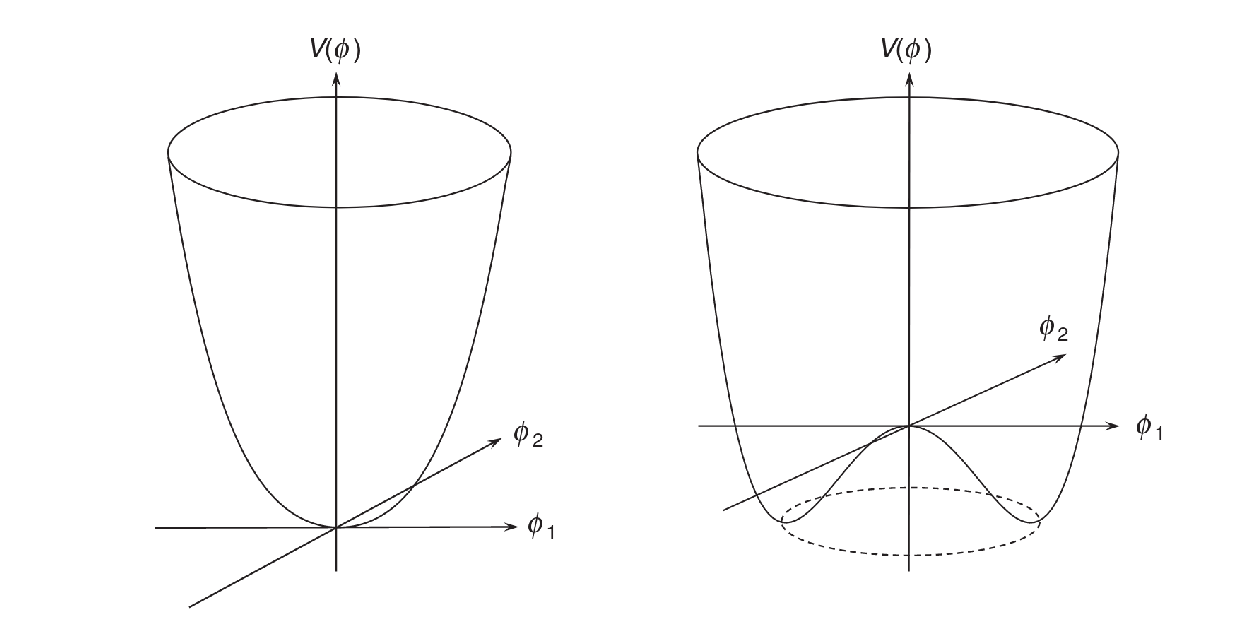
\includegraphics[width=.65\linewidth]{Figures/theory/higgs_potential.pdf}
  \caption[The Higgs potential]
  {
    The potential, $V(\phi)$, for a single complex scalar field, $\phi=\frac{1}{\sqrt{2}}(\phi_1+i\phi_2)$, uniquely defined by the parameters: $\mu^2$ and $\lambda$. The plot on the left shows the scenario for $\mu^2>0$ and $\lambda>0$, whilst the plot on the right shows the scenario for $\mu^2<0$ and $\lambda>0$. It is the form on the right which is required for SSB via the HEB mechanism. Figure taken from Ref.~\cite{Thomson:2013zua}.
  }
  \label{fig:higgs_potential}
\end{figure}

We can extend this idea to the Higgs doublet with four degrees of freedom, where the non-zero vacuum states satisfy,

\begin{equation}
    H^{\dagger}H = \frac{1}{2}(\phi_1^2+\phi_2^2+\phi_3^2+\phi_4^2) = -\frac{\mu^2}{2\lambda} = \frac{v^2}{2}.
\end{equation}

\noindent
To achieve the SSB expressed in equation~\ref{eq:ssb}, a vacuum state is chosen to generate the masses of the ${\rm{W}}^\pm$ and Z bosons, whilst leaving the symmetry of the electromagnetic (EM) interaction intact, and therefore the photon massless. This choice~\cite{Weinberg:1967tq} is,

\begin{equation}
    \langle 0 | H | 0 \rangle = \frac{1}{\sqrt{2}}\begin{pmatrix}
    0 \\
    v
    \end{pmatrix},
\end{equation}

\noindent
where $v=\sqrt{-\mu^2/\lambda}$ is the Higgs field vacuum expectation value. We then consider non-linear perturbations about this minimum of the form,

\begin{equation}
    H = e^{iG^i(x)\frac{\sigma^i}{2}} \cdot \frac{1}{\sqrt{2}}\begin{pmatrix}
    0 \\
    v + h(x)
    \end{pmatrix}
\end{equation}

\noindent
where the Goldstone theorem~\cite{Goldstone:1962es} predicts the existence of three massless Goldstone boson fields, $G^i(x)$, for each broken generator of the symmetry group, and one massive scalar boson, $h(x)$, for the unbroken symmetry. The Goldstone bosons can be eliminated from the Lagrangian by making the appropriate local gauge transformation,

\begin{equation}
    {\rm{SU}(2)}_{\rm{L}}: H \mapsto H' = e^{i\theta^i(x)\frac{\sigma^i}{2}}H
\end{equation}

\noindent
and choosing $\theta^i(x)=\frac{-G(x)^i}{v}$\footnote{It is important to keep in mind that we are free to make this choice, since the underlying Lagrangian is invariant under local gauge transformations.}. This is known as the \textit{unitary gauge}, where the Higgs doublet field takes the form,

\begin{equation}
    H = \frac{1}{\sqrt{2}}\begin{pmatrix}
    0 \\
    v + h(x)
    \end{pmatrix}
\end{equation}

\noindent
Crucially, the three degrees of freedom corresponding to the massless Goldstone boson fields no longer appear in the Lagrangian. Instead, due to the covariant derivative in $\mathcal{L}_{\rm{Higgs}}$, they are absorbed as the longitudinal polarisation states of the weak vector bosons: ${\rm{W}}^{\pm}$ and Z. This is explicitly shown by inserting $H$ in the unitary gauge into equation~\ref{eq:higgs_term}, where we find the following terms,

\begin{equation}
    \mathcal{L}_{\rm{Higgs}} \supset \frac{1}{4}g^2v^2W^{+\mu}W^-_\mu + \frac{1}{8}v^2(g^2+g'^2)Z^{\mu}Z_\mu.
\end{equation}

\noindent
These are directly the weak boson mass terms that we set out to achieve. By introducing the HEB mechanism into the SM, we have successfully generated the masses of the weak bosons via the spontaneous symmetry breaking of the EW interaction. Using the known form of a mass term for a spin-1 gauge boson ($m_W^2 W_\mu W^\mu$), we read off the ${\rm{W}}^{\pm}$ and Z boson masses as,

\begin{equation}
    m_W = \frac{1}{2}gv = 80.4\;{\rm{GeV}}, \qquad m_Z = \frac{v}{2}\sqrt{g^2+g'^2} = 91.2\;{\rm{GeV}},
\end{equation}

\noindent
which depend on the Higgs vacuum expectation value, $v=246$~GeV, and the coupling strengths of the ${\rm{SU}(2)_{\rm{L}}}\otimes{\rm{U}}(1)_{\rm{Y}}$ EW interaction. Remarkably, no equivalent mass term exists for the $A^\mu$ field: the photon remains massless. This is exactly what is required for a consistent description of the weak and electromagnetic interactions.

The Lagrangian also contains the following terms,
\begin{equation}\label{eq:scalar_lagrangian}
    \mathcal{L}_{\rm{Higgs}} \supset \frac{1}{2}(\partial_\mu h)(\partial^\mu h) + \lambda v^2 h^2 -{\lambda}vh^3 -\frac{1}{4}\lambda h^4.
\end{equation}
\noindent
which describe an additional massive scalar boson field, h, with mass $m_H=\sqrt{2\lambda}v$\footnote{The (seemingly poor) choice in notation in using $m_H$ instead of $m_h$, is simply made because $m_H$ is more commonly used in the literature.}. The quantum excitation of this field, the Higgs boson, was discovered by the ATLAS and CMS Collaborations in 2012~\cite{Aad:2012tfa,Chatrchyan:2012xdj,Chatrchyan:2013lba}, with a mass of around 125~GeV. 

The final two terms in equation~\ref{eq:scalar_lagrangian} describe the trilinear and quartic self-interactions of the Higgs boson, which are shown as Feynman diagrams on the left of Figure~\ref{fig:feynman_higgs_interactions}. Such interactions are extremely rare and have not yet been observed in high energy physics experiments. In the SM, the value of $\lambda$ is uniquely defined by the relation $m_H=\sqrt{2\lambda}v$, nevertheless, the presence of BSM physics can modify $\lambda$ without changing the values of $m_H$ and $v$. Measurements of the Higgs boson self-interactions are therefore in high demand as they provide an independent probe of $\lambda$; from which we can infer the shape of the Higgs potential, and subsequently the dynamics of EW symmetry breaking. Chapter~\ref{chap:hllhc} investigates an indirect method for probing $\lambda$ at a future operation of the LHC machine.

Additionally, the $(D^\mu H)^{\dagger}(D_\mu H)$ term in $\mathcal{L}_{\rm{Higgs}}$ gives rise to terms $\propto {\rm{VV}}h$ and ${\propto {\rm{VV}}h^2}$, where ${\rm{V}}={\rm{W}}^{\pm},{\rm{Z}}$. These correspond to the triple and quartic couplings between the weak bosons and the Higgs boson, as shown on the right of Figure~\ref{fig:feynman_higgs_interactions}. The coupling strength at the $h{\rm{W^+W^-}}$ vertex is equal to $\frac{1}{2}g^2v \equiv g\,m_W$; the coupling of the Higgs boson to the W boson is proportional to the W boson mass. The equivalent is true for the $h{\rm{ZZ}}$ vertex, where the coupling strength is $\propto m_Z$. No coupling exists between the $h$ and the photon field, $A_\mu$, nor does $h$ couple to the gluon field, $G^a_\mu$.

\begin{figure}[htb!]
  \centering
  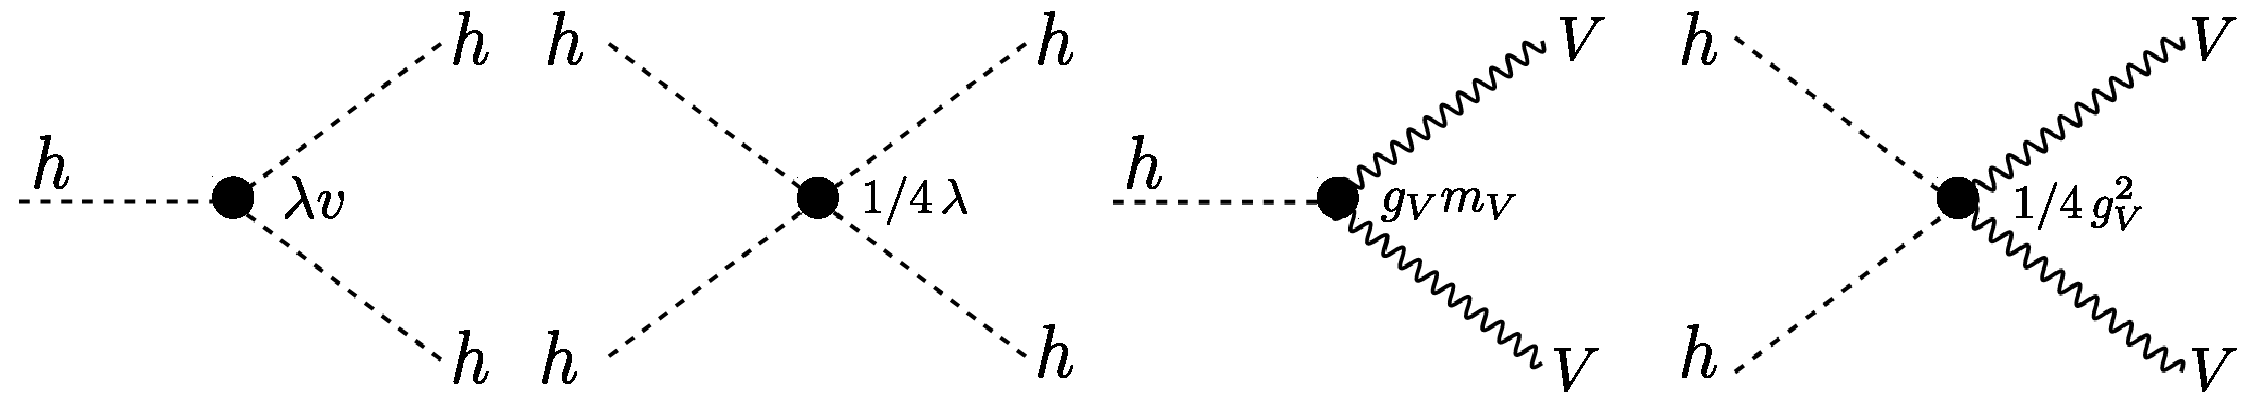
\includegraphics[width=.9\linewidth]{Figures/theory/higgs_interaction.pdf}
  \caption[The Higgs boson interactions]
  {
    The Higgs boson self-interactions (left) and the Higgs boson interactions with the weak gauge bosons (right). The couplings $g_V=g_W$ and $g_Z$ are equal to $g$ and $g/\cos{\theta_W}$, respectively.
  }
  \label{fig:feynman_higgs_interactions}
\end{figure}

\subsubsection{Yukawa interactions}
The fermion masses are generated in the SM via the Yukawa interactions~\cite{Thomson:2013zua}. The following ${\rm{SU}(2)_{\rm{L}}}\otimes{\rm{U}}(1)_{\rm{Y}}$ gauge invariant terms are added to the SM Lagrangian,

\begin{equation}\label{eq:yukawa}
    \mathcal{L}_{\rm{SM}} \supset \mathcal{L}_{\rm{Yukawa}} = -(\lambda_j \bar{L}_{jL} H \ell_{jR} + \lambda_j \bar{Q}^a_{jL} H d^a_{jR} + \lambda_j \bar{Q}^a_{jL} \tilde{H} u^a_{jR} + {\rm{h.c.}})
\end{equation}

\noindent
where $\lambda_j$ are the Yukawa couplings for fermion flavour state, $j$, the notation $\tilde{H}^k=\epsilon_{kl}(H^l)^*$ is used, where $\epsilon_{jk}$ is totally antisymmetric in its indices with $\epsilon_{12}=+1$, and ${\rm{h.c.}}$ are the hermitian conjugates of the explicitly written terms. After SSB (substituting the unitary gauge $H$ doublet into equation~\ref{eq:yukawa}) we find terms of the form,

\begin{equation}
   \mathcal{L}_{\rm{Yukawa}} \subset -\frac{\lambda_e}{\sqrt{2}}v(\bar{e}_Le_R+\bar{e}_Re_L)-\frac{\lambda_e}{\sqrt{2}}h(\bar{e}_Le_R+\bar{e}_Re_L),
\end{equation}

\noindent
where for simplicity, only the terms relevant for the electron field are shown. The first term has exactly the form required for fermion masses, $m_{j}(\bar{\psi}_{jL}\psi_{jR}+\bar{\psi}_{jR}\psi_{jL})$, from which we can infer the relation, $\lambda_j = \sqrt{2}m_j/v$. The second term represents the couplings of the fermions fields to the Higgs boson: $h\bar{\psi}\psi$. These interactions have a coupling strength proportional to $\lambda_j$, and therefore the Higgs boson coupling to fermions is directly proportional to the mass of the fermion field. Whilst the HEB mechanism does not predict the values of $\lambda_j$, the masses of the fermions are measured experimentally, and hence provide a handle on the coupling properties of the Higgs boson.

\subsection{The SM Lagrangian}
Putting everything together, we arrive at an expression for the ${\rm{SU}}(3)_{\rm{C}} \otimes {\rm{SU}}(2)_{\rm{L}} \otimes {\rm{U}}(1)_{\rm{Y}}$ gauge invariant SM Lagrangian (before SSB) to be,

\begin{equation}
\begin{split}
    \mathcal{L}_{\rm{SM}} = & \mathcal{L}_{\rm{gauge}} + \mathcal{L}_{\rm{Higgs}} + \mathcal{L}_{\rm{int}} + \mathcal{L}_{\rm{Yukawa}}
    \\
    = &-\frac{1}{4}G^a_{\mu\nu}G^{a,\mu\nu} -\frac{1}{4}W^i_{\mu\nu}W^{i,\mu\nu} -\frac{1}{4}B_{\mu\nu}B^{\mu\nu} 
    \\
    &+ (D^\mu H)^{\dagger}(D_\mu H) - \mu^2H^{\dagger}H - \frac{1}{4}\lambda(H^{\dagger}H)^2
    \\
    &+ i(\bar{L}\slashed{D}L+\bar{\ell}\slashed{D}\ell+\bar{Q}\slashed{D}Q+\bar{u}\slashed{D}u+\bar{d}\slashed{D}d)
    \\
    &- (\lambda_\ell \bar{L} H \ell + \lambda_d \bar{Q} H d + \lambda_u \bar{Q} \tilde{H} u + {\rm{h.c.}})
\end{split}
\end{equation}

\noindent
where the colour, flavour and chirality indices ($L$,$R$) have been dropped from the fermion fields in the notation, and $\lambda_{\ell,u,d}$ are now matrices in the flavour space. The covariant derivative, $D_\mu$, which maintains the gauge invariance, is,

\begin{equation}
    D_\mu = \partial_\mu + i g_s G^a_\mu \frac{\lambda^a}{2} + i g W^i_\mu \frac{\sigma^i}{2} + i g' B_\mu {\rm{Y}}
\end{equation}

\noindent
where the $G^a_\mu$, $W^i_\mu$ and $B_\mu$ terms act on the fields with non-zero colour charge, non-zero weak isospin ($t_3$) and non-zero weak hypercharge ($y$), respectively. Incredibly, this Lagrangian density which barely spans four lines encompasses all known particle interactions via the electromagnetic, strong and weak forces, and with the inclusion of the HEB mechanism, explains how the weak gauge boson and fermion fields\footnote{This does not include the generation of neutrino masses which requires a separate mechanism. The mechanism will not be discussed here since it is not relevant for this thesis.} acquire mass. The pillars of the theory that have lead to the construction of $\mathcal{L}_{\rm{SM}}$ are summarised in Figure~\ref{fig:sm_pillars}.

\begin{figure}[htb!]
  \centering
  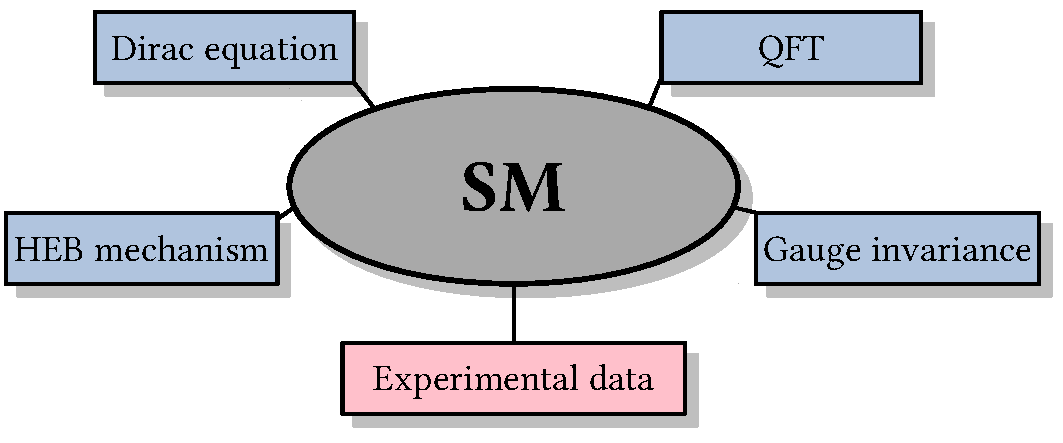
\includegraphics[width=.7\linewidth]{Figures/theory/pillars_of_sm.pdf}
  \caption[The pillars of SM theory]
  {
    The pillars of SM theory.
  }
  \label{fig:sm_pillars}
\end{figure}

One expects the ultimate theory of particle physics to be described by a simple equation with few free parameters~\cite{Thomson:2013zua}; plainly, the SM is \textit{not} this theory. Despite being constructed from a number of profound theoretical ideas (blue boxes), it is put together in a somewhat ad-hoc manner. This becomes clear when considering the relatively large number of free parameters in the model (26 in total) which are independently tuned to match experimental observations (red box). Table~\ref{tab:sm_freeparams} lists the free parameters of the SM.

\begin{table}[htb]
    \caption[The free parameters of the SM]{The 26 free parameters of the SM, which are input directly from experiment. References are provided for the parameters associated with topics that have not been addressed in the text.}
    \label{tab:sm_freeparams}
    \centering
    \footnotesize
    \renewcommand{\arraystretch}{2}
    \begin{tabular}{r|l}
       Fermion masses & $m_u$, $m_c$, $m_t$, $m_d$, $m_s$, $m_b$, $m_e$, $m_\mu$, $m_\tau$, $m_{{\nu}1}$, $m_{{\nu}2}$, $m_{{\nu}3}$ \\
       Gauge interaction coupling strengths & $g$, $g'$, $g_s$ \\
       HEB mechanism & $v$, $m_H$ \\
       CKM and PMNS mixing angles~\cite{Cabibbo:1963yz,Kobayashi:1973fv,Pontecorvo:1957qd,Maki:1962mu} & $\lambda$, $A$, $\rho$, $\eta$, $\theta_{12}$, $\theta_{13}$, $\theta_{23}$, $\delta$  \\
       Strong CP phase~\cite{strongcp} & $\theta^{\rm{CP}}(\approx0)$\\
    \end{tabular}
\end{table}

Given this set of input parameters, all the SM particle masses and couplings are fully predicted. For example, the $\lambda$ parameter which appears in the definition of the Higgs potential is equal to $m_H^2/2v^2$. Nevertheless, the presence of new BSM fields can modify the SM predictions, and thus leave an imprint on the masses and couplings of the SM fields. In turn, this affects not only the rate of interesting collision events at the LHC, but also their kinematic properties\footnote{For example, an additional high mass state decaying to a Higgs boson will enhance the Higgs boson production rate at high momentum.}. Altogether, this provides a concrete tool to search for new physics: by precisely measuring the masses and couplings of the SM fields and checking for consistency with the SM theory, we can indirectly infer the presence of new BSM states. In this thesis, we investigate the precision measurements of Higgs boson properties at the CMS experiment.

\section{Higgs boson phenomenology}
This section describes how the SM predictions manifest in terms of the Higgs boson phenomenology at a hadron collider. As mentioned at the beginning of this chapter, in high energy particle collision experiments we do not observe the fundamental fields, but instead infer their interactions via production cross sections, $\sigma$, and decay rates, $\Gamma$. These observables are mapped back to the parameters of the model Lagrangian by computing the relevant matrix element, $\mathcal{M}_{i \rightarrow f}$: a quantity which encodes the probability of the transition from initial state, $i$, to final state, $f$, as a function of the particle couplings and masses. A useful introduction to the calculation of matrix elements (using the Feynman rules) is left to Ref.~\cite{Thomson:2013zua}. 

\subsubsection{Higgs boson production}
For proton-proton collisions at a centre-of-mass energy of $\sqrt{s}=13$~TeV, the four major Higgs boson production modes are (in order of decreasing cross section): gluon-gluon fusion (ggH), vector boson fusion (VBF), vector boson associated production (VH), and production in association with a top quark-antiquark pair (ttH)\footnote{From now on the distinction between fermions and anti-fermions is left out of the notation. For example, ttH strictly represents t$\bar{\rm{t}}$H production. Additionally, the V in VBF and VH includes both W and Z bosons: ${\rm{V}}={\rm{W}}^{\pm},{\rm{Z}}$.}. All such production modes are now observed with significance $>$5$\sigma$ at the LHC~\cite{CMS-PAS-HIG-19-005,Aad:2019mbh}. Additionally, there are a number of rarer production modes including single-top associated production (tH), gluon-initiated Z boson associated production (ggZH), and production in association with a bottom quark-antiquark pair (bbH). The leading order\footnote{See section~\ref{sec:mc}.} Feynman diagrams for all the aforementioned Higgs boson production modes are displayed in Figure~\ref{fig:higgs_production_feynman}, and the expected SM cross sections for each process are listed in Table~\ref{tab:higgs_xs}. These values correspond to a nominal Higgs boson mass of $m_H=125.0$~GeV.

\begin{figure}[htb!]
  \centering
  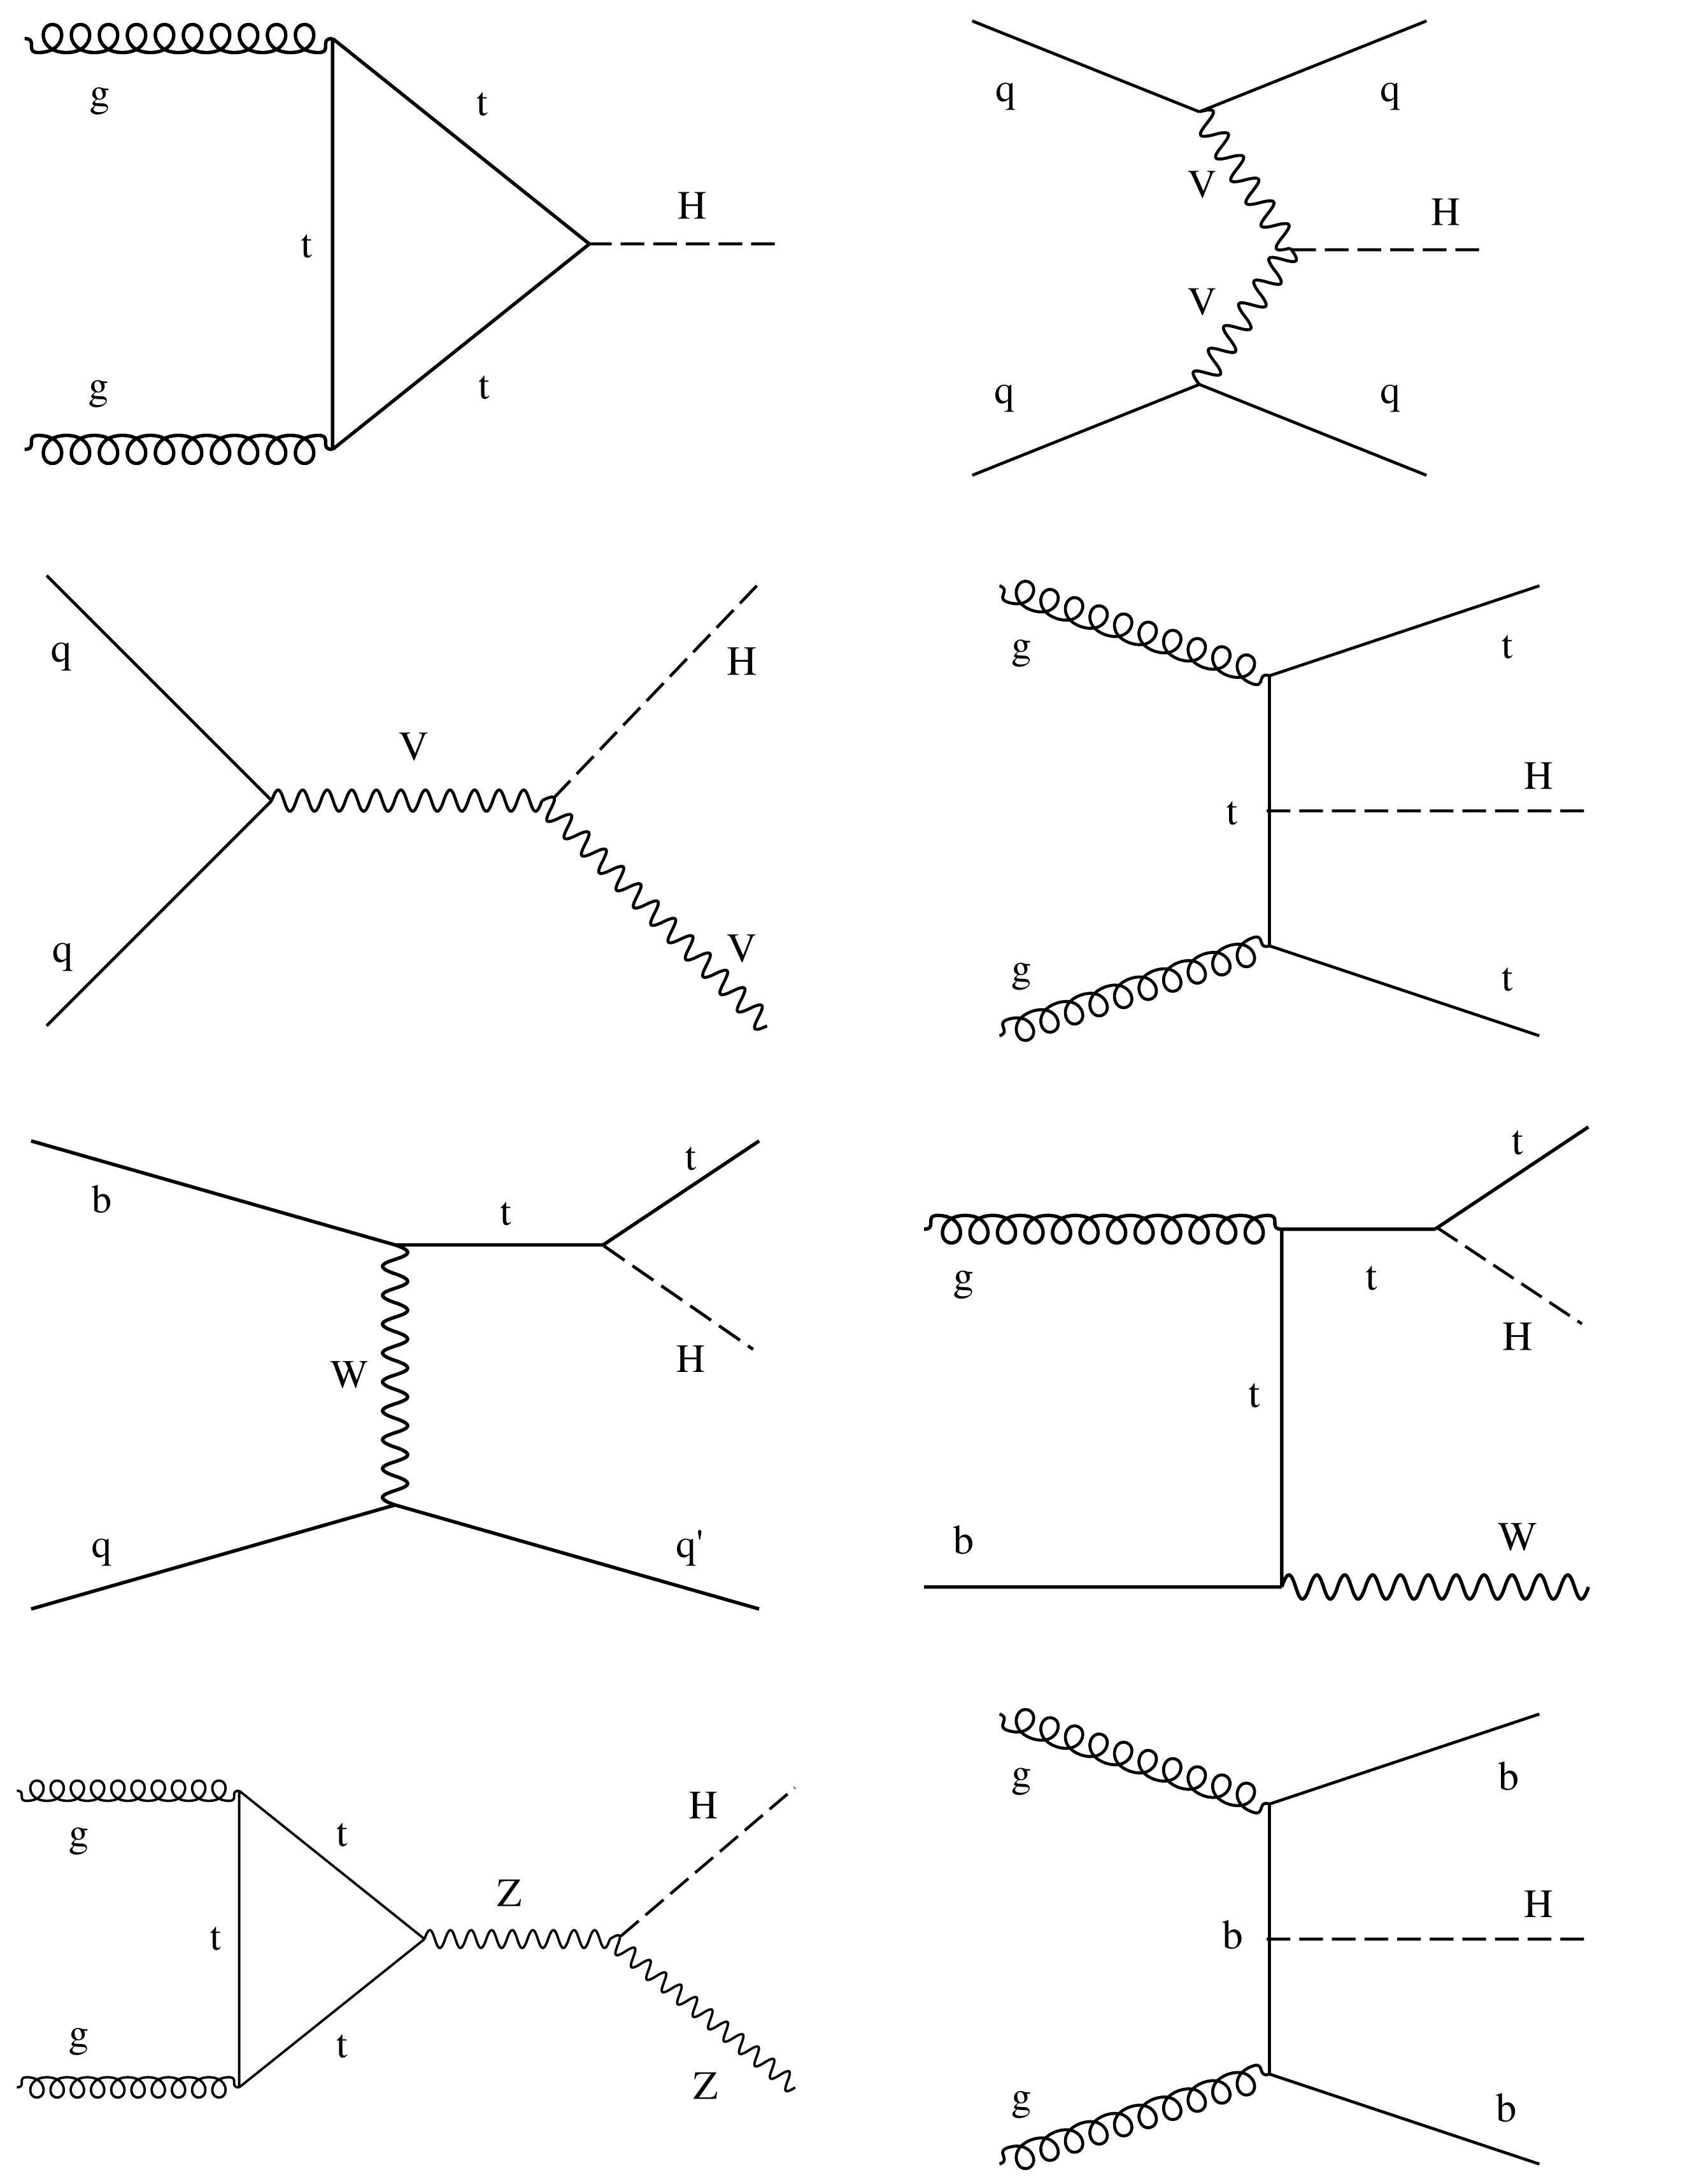
\includegraphics[width=.8\linewidth]{Figures/theory/production_feynman.png}
  \caption[Leading order Feynman diagrams for the major Higgs boson production modes]
  {
    Example leading order Feynman diagrams for the major Higgs boson production modes at the LHC: ggH (top left), VBF (top right), VH (second left), ttH (second right), tHq (third left), tHW (third right), ggZH (bottom left) and bbH (bottom right).
  }
  \label{fig:higgs_production_feynman}
\end{figure}

\begin{table}[htb]
    \caption[Higgs boson production cross sections]{SM Higgs boson production cross sections at $\sqrt{s}=13$~TeV, for $m_H=125.0$~GeV. The VH and tH production modes are separated into the contributions from the WH and ZH modes, and tHq and tHW modes, respectively. Values are taken from Ref.~\cite{deFlorian:2016spz}.}
    \label{tab:higgs_xs}
    % \vspace{.5cm}
    \centering
    \footnotesize
    \setlength{\tabcolsep}{8pt}
    \renewcommand{\arraystretch}{2}
    \begin{tabular}{l|c|c|c|c|c|c|c|c|c}
        Production mode & ggH & VBF & WH & ZH & ggZH & ttH & tHq & tHW & bbH   \\ \hline
        Cross section [pb] & 48.6 & 3.78 & 1.37 & 0.76 & 0.12 & 0.51 & 0.077 & 0.015 & 0.49 \\
    \end{tabular}
\end{table}

The ggH production mode proceeds via an internal quark loop as the Higgs boson does not directly couple to the gluon (g). This makes ggH particularly sensitive to new physics where the quarks in the loop could in principle be replaced by a heavy BSM state that couples to the Higgs boson. In the SM, the cross section of ggH dominates by roughly an order of magnitude. Nevertheless, the other modes contain additional objects in their final states which can help identify them from other SM background processes. For example, VBF events are typically characterised by two additional jets, produced from the final-state quarks, with a large angular separation. Ultimately, the experimental sensitivity to a particular production mode depends on both the cross section and the degree of background contamination mimicking the signal process.

\subsubsection{Higgs boson decay}
The Higgs boson is an unstable particle with a very short lifetime~\cite{Zyla:2020zbs}. Consequently, it decays instantaneously and can only be inferred from the observation of its decay products. The principal Higgs boson decay channels are listed with their respective branching fractions, $\mathcal{B}^f$, for $m_H=125.0$~GeV in Table~\ref{tab:higgs_br}, where $\mathcal{B}^f=\Gamma^f/\Gamma^H$, and $\Gamma^H$ is the total decay width of the Higgs boson.

\begin{table}[htb]
    \caption[Higgs boson decay branching fractions]{Higgs boson decay branching fractions for $m_H=125.0$~GeV. Values are taken from Ref.~\cite{deFlorian:2016spz}.}
    \label{tab:higgs_br}
    % \vspace{.5cm}
    \centering
    \footnotesize
    \setlength{\tabcolsep}{8pt}
    \renewcommand{\arraystretch}{2}
    \begin{tabular}{l|c|c|c|c|c|c|c|c}
        Decay channel & bb & WW$^{*}$ & gg & $\tau\tau$ & cc & ZZ$^{*}$ & $\gamma\gamma$ & $\mu\mu$   \\ \hline
        Branching fraction [\%] & 58.2 & 21.4 & 8.2 & 6.3 & 2.8 & 2.6 & 0.23 & 0.022  \\
    \end{tabular}
\end{table}

The dominant Higgs boson decay channel is \Hbb, which occurs via the direct Yukawa coupling of the Higgs boson to the bottom quark. Nevertheless, the \Hbb decay channel was only recently observed during Run 2 of the LHC~\cite{Aaboud:2018zhk,Sirunyan:2018kst} due to the large hadronic background at the LHC. Other decay channels with relatively low branching fractions (e.g. \Hfl, \Hgg) offer greater sensitivity to Higgs boson measurements. Of particular interest in this thesis is the \Hgg decay channel. This channel benefits from a clean final state topology of two well-reconstructed photons, that provide a narrow invariant mass (\mgg) peak about the Higgs boson mass, $m_H$. This property is used to effectively distinguish \Hgg events from the smoothly-falling background continuum. Moreover, it is one of the few channels that is sensitive to all of the major Higgs boson production modes.

\begin{figure}[htb!]
  \centering
  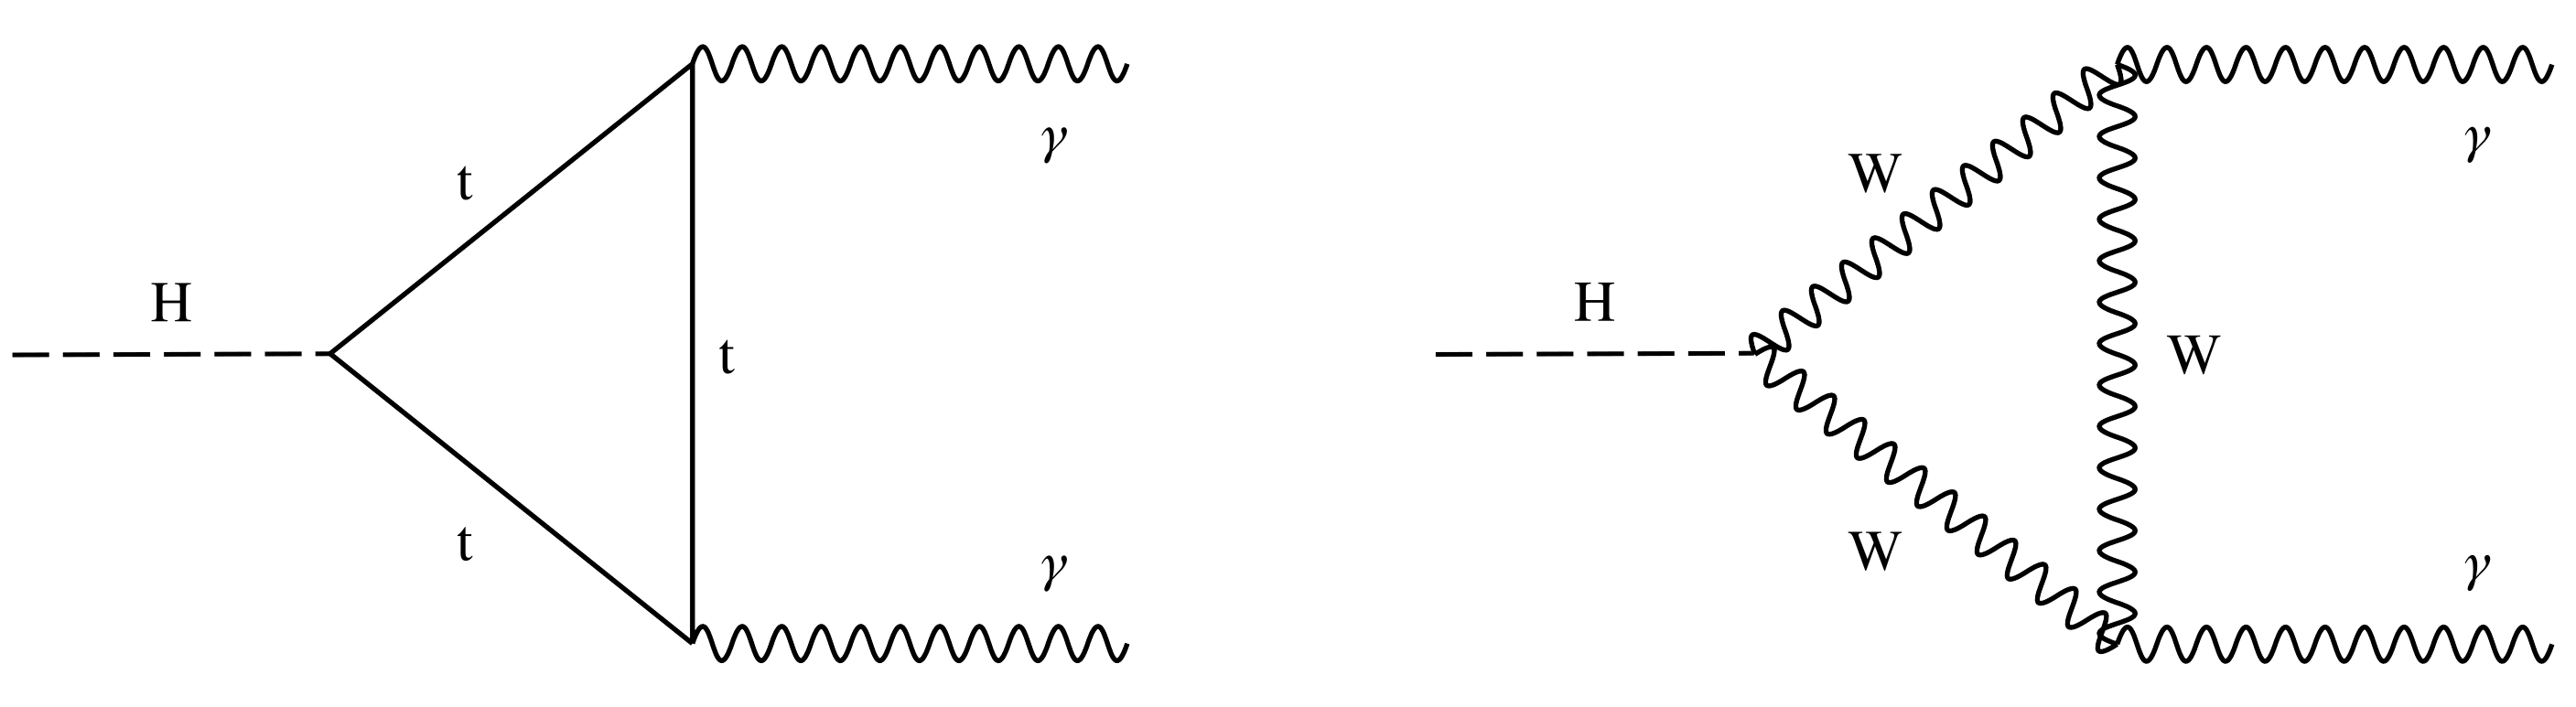
\includegraphics[width=.8\linewidth]{Figures/theory/hgg_decay_feynman.png}
  \caption[Leading order Feynman diagrams for the \Hgg decay channel]
  {
    Leading order Feynman diagrams for the \Hgg decay channel.
  }
  \label{fig:hgg_decay}
\end{figure}

Two of the leading-order Feynman diagrams for \Hgg in the SM are displayed in Figure~\ref{fig:hgg_decay}. Like ggH production, the \Hgg decay proceeds via an internal loop as the Higgs boson does not couple directly to the photon field. This loop includes contributions from both top quarks and ${\rm{W}}^{\pm}$ bosons, meaning the \Hgg decay rate is sensitive to both the top Yukawa coupling and the Higgs-W boson coupling, respectively.

\subsubsection{Previous \Hgg result at CMS}
At this point, it would be cumbersome to review all results from the \Hgg decay channel at CMS, let alone from all decay channels. In preparation for the following section, it is useful to introduce a single result from the \Hgg decay channel, which uses proton-proton collision data collected during the 2016 period~\cite{Sirunyan:2018ouh}. Figure~\ref{fig:hig16040_stage0} shows the measurement of the dominant Higgs boson production mode cross sections relative to their SM predictions. The VH production mode is separated according to the decay of the vector boson: leptonic (${\rm{Z}}\rightarrow\ell\ell/\nu\nu$ and ${\rm{W}}\rightarrow\ell\nu$) and hadronic (${\rm{W/Z}}\rightarrow qq'/qq$), and the leptonic channel is further divided into the WH and ZH production contributions. With the 2016 data only, the ggH cross section is measured to within an uncertainty of around 20\%. Other production modes are measured less well, with uncertainties ranging from 50-60\% for VBF production to 250\% for VH hadronic. Looking forward, the inclusion of more data will help reduce the statistical uncertainty in these measurements, and will enable new, more granular measurements to be made. One framework for performing such granular measurements is the \textit{simplified template cross section} (STXS) framework.

\begin{figure}[htb!]
  \centering
  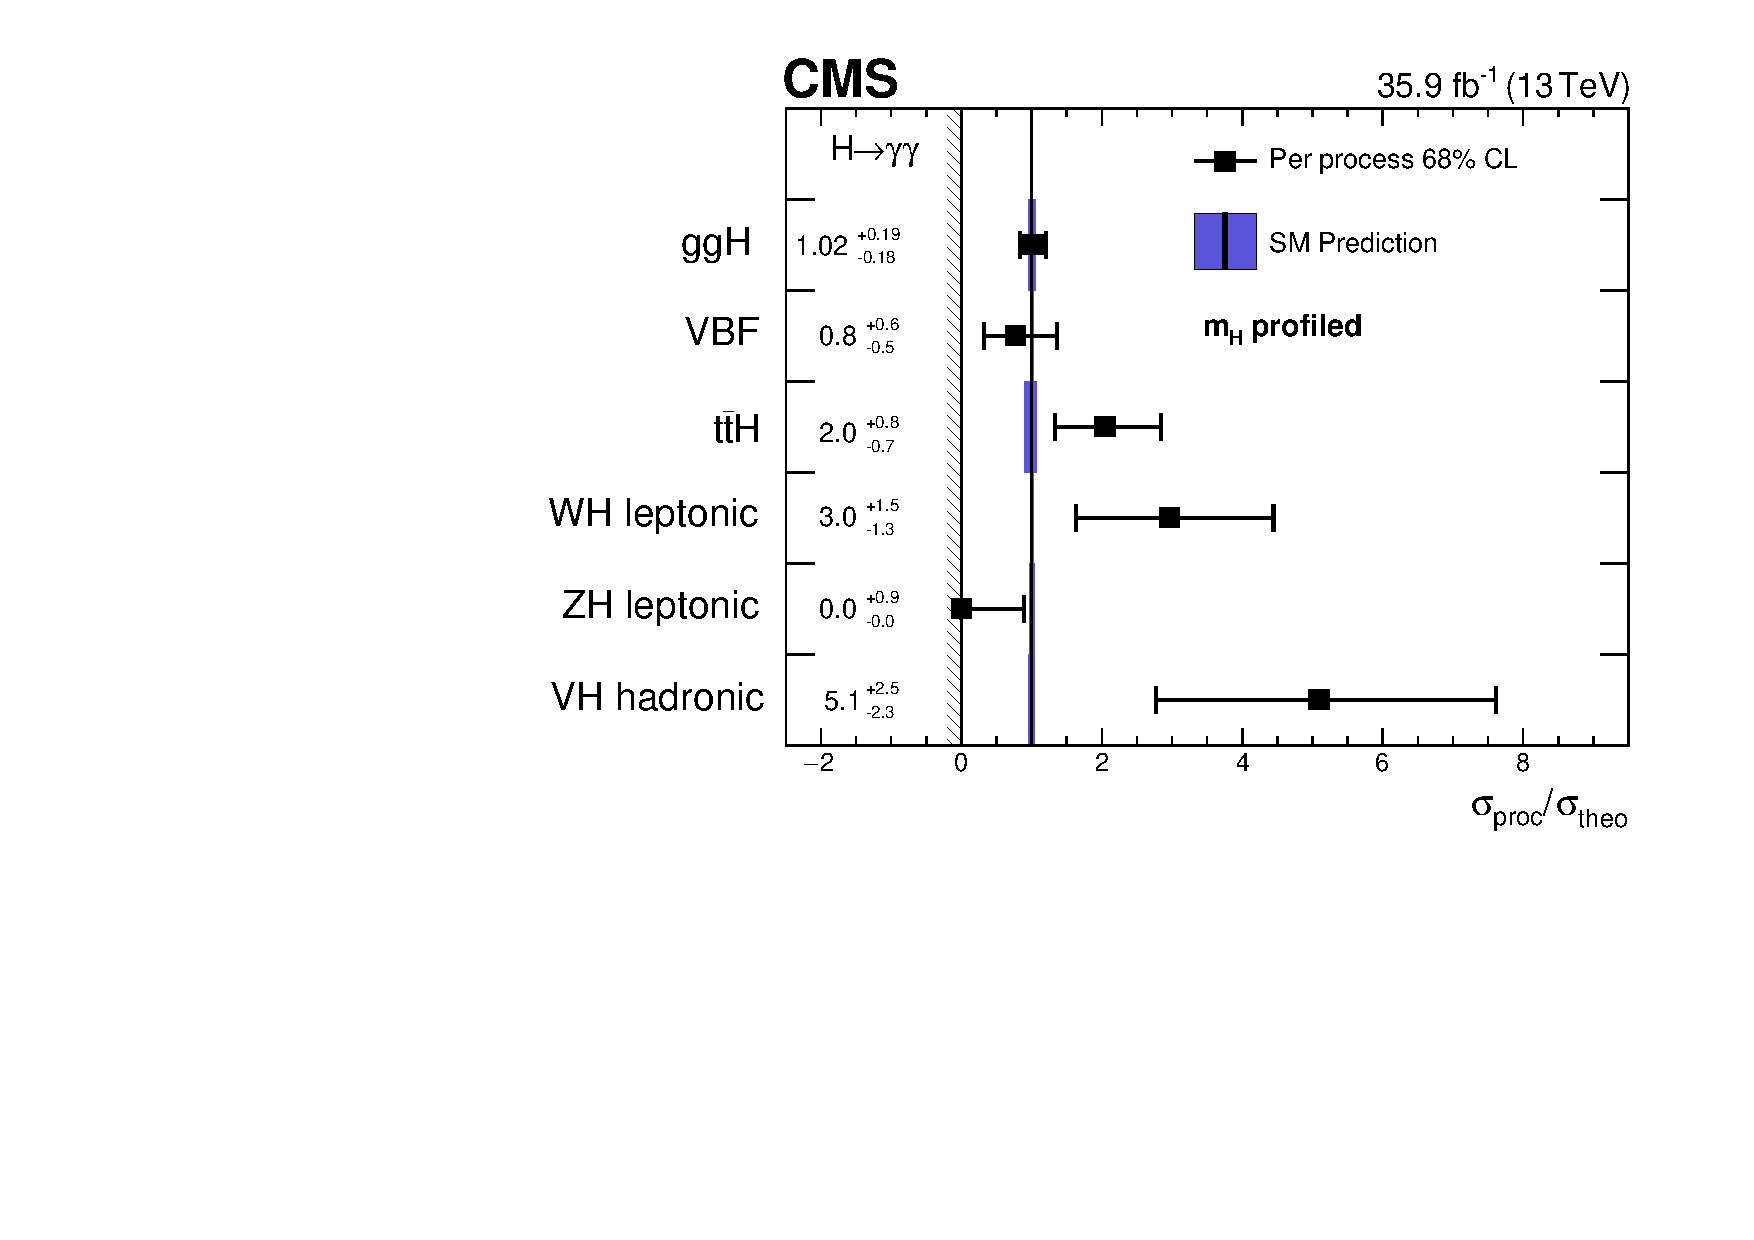
\includegraphics[width=.7\linewidth]{Figures/theory/hig16040_stage0.pdf}
  \caption[Measurements of Higgs boson production cross section in the \Hgg channel, using the 2016 data set]
  {
    Measurements of the dominant Higgs boson production mode cross sections, relative to their SM predictions, in the \Hgg decay channel. The results use data collected by the CMS experiment during the 2016 data taking period. The black points represent the best-fit values and 68\% confidence intervals for the measured parameters of interest. The blue boxes demonstate the theoretical uncertainties in the SM predictions.
  }
  \label{fig:hig16040_stage0}
\end{figure}

\section{Simplified template cross sections}\label{sec:theory_stxs}
The STXS framework~\cite{deFlorian:2016spz} is a remarkably simple concept: as the available data increases, we divide the Higgs boson production phase space into increasingly granular kinematic regions. These regions, or so-called \textit{bins}, are split primarily by the Higgs boson production mode and subsequently by the kinematic quantities of the event. The framework provides a natural progression to inclusive production mode measurements (see Figure~\ref{fig:hig16040_stage0}), such that by measuring the cross section in the kinematic regions, we build up a more granular description of Higgs boson production, and gain an understanding of the event kinematics. Ultimately, this enhances the sensitivity to potential new physics contributions that appear in specific regions of the Higgs boson production phase space.

This coherent approach to precision Higgs boson measurements has been adopted by the ATLAS and CMS Collaborations for a number of years. The evolution of the framework with increasing statistics is defined in so-called \textit{stages}~\cite{deFlorian:2016spz,Berger:2019wnu}, which refer to different kinematic binning schemes of varying granularity. The \Hgg analysis documented in chapters~\ref{chap:hgg_overview}--\ref{chap:hgg_results} targets the most-granular stage 1.2 binning definition, which is shown schematically in Figure~\ref{fig:stxs_schematic}. The effective field theory interpretation of STXS measurements in chapter~\ref{chap:eft} combines cross section measurements from different Higgs boson decay channels at stage 0, stage 1.0 and stage 1.1. All stages are displayed schematically in Appendix~\ref{app:merging_schemes}.

\begin{figure}[htb!]
  \centering
  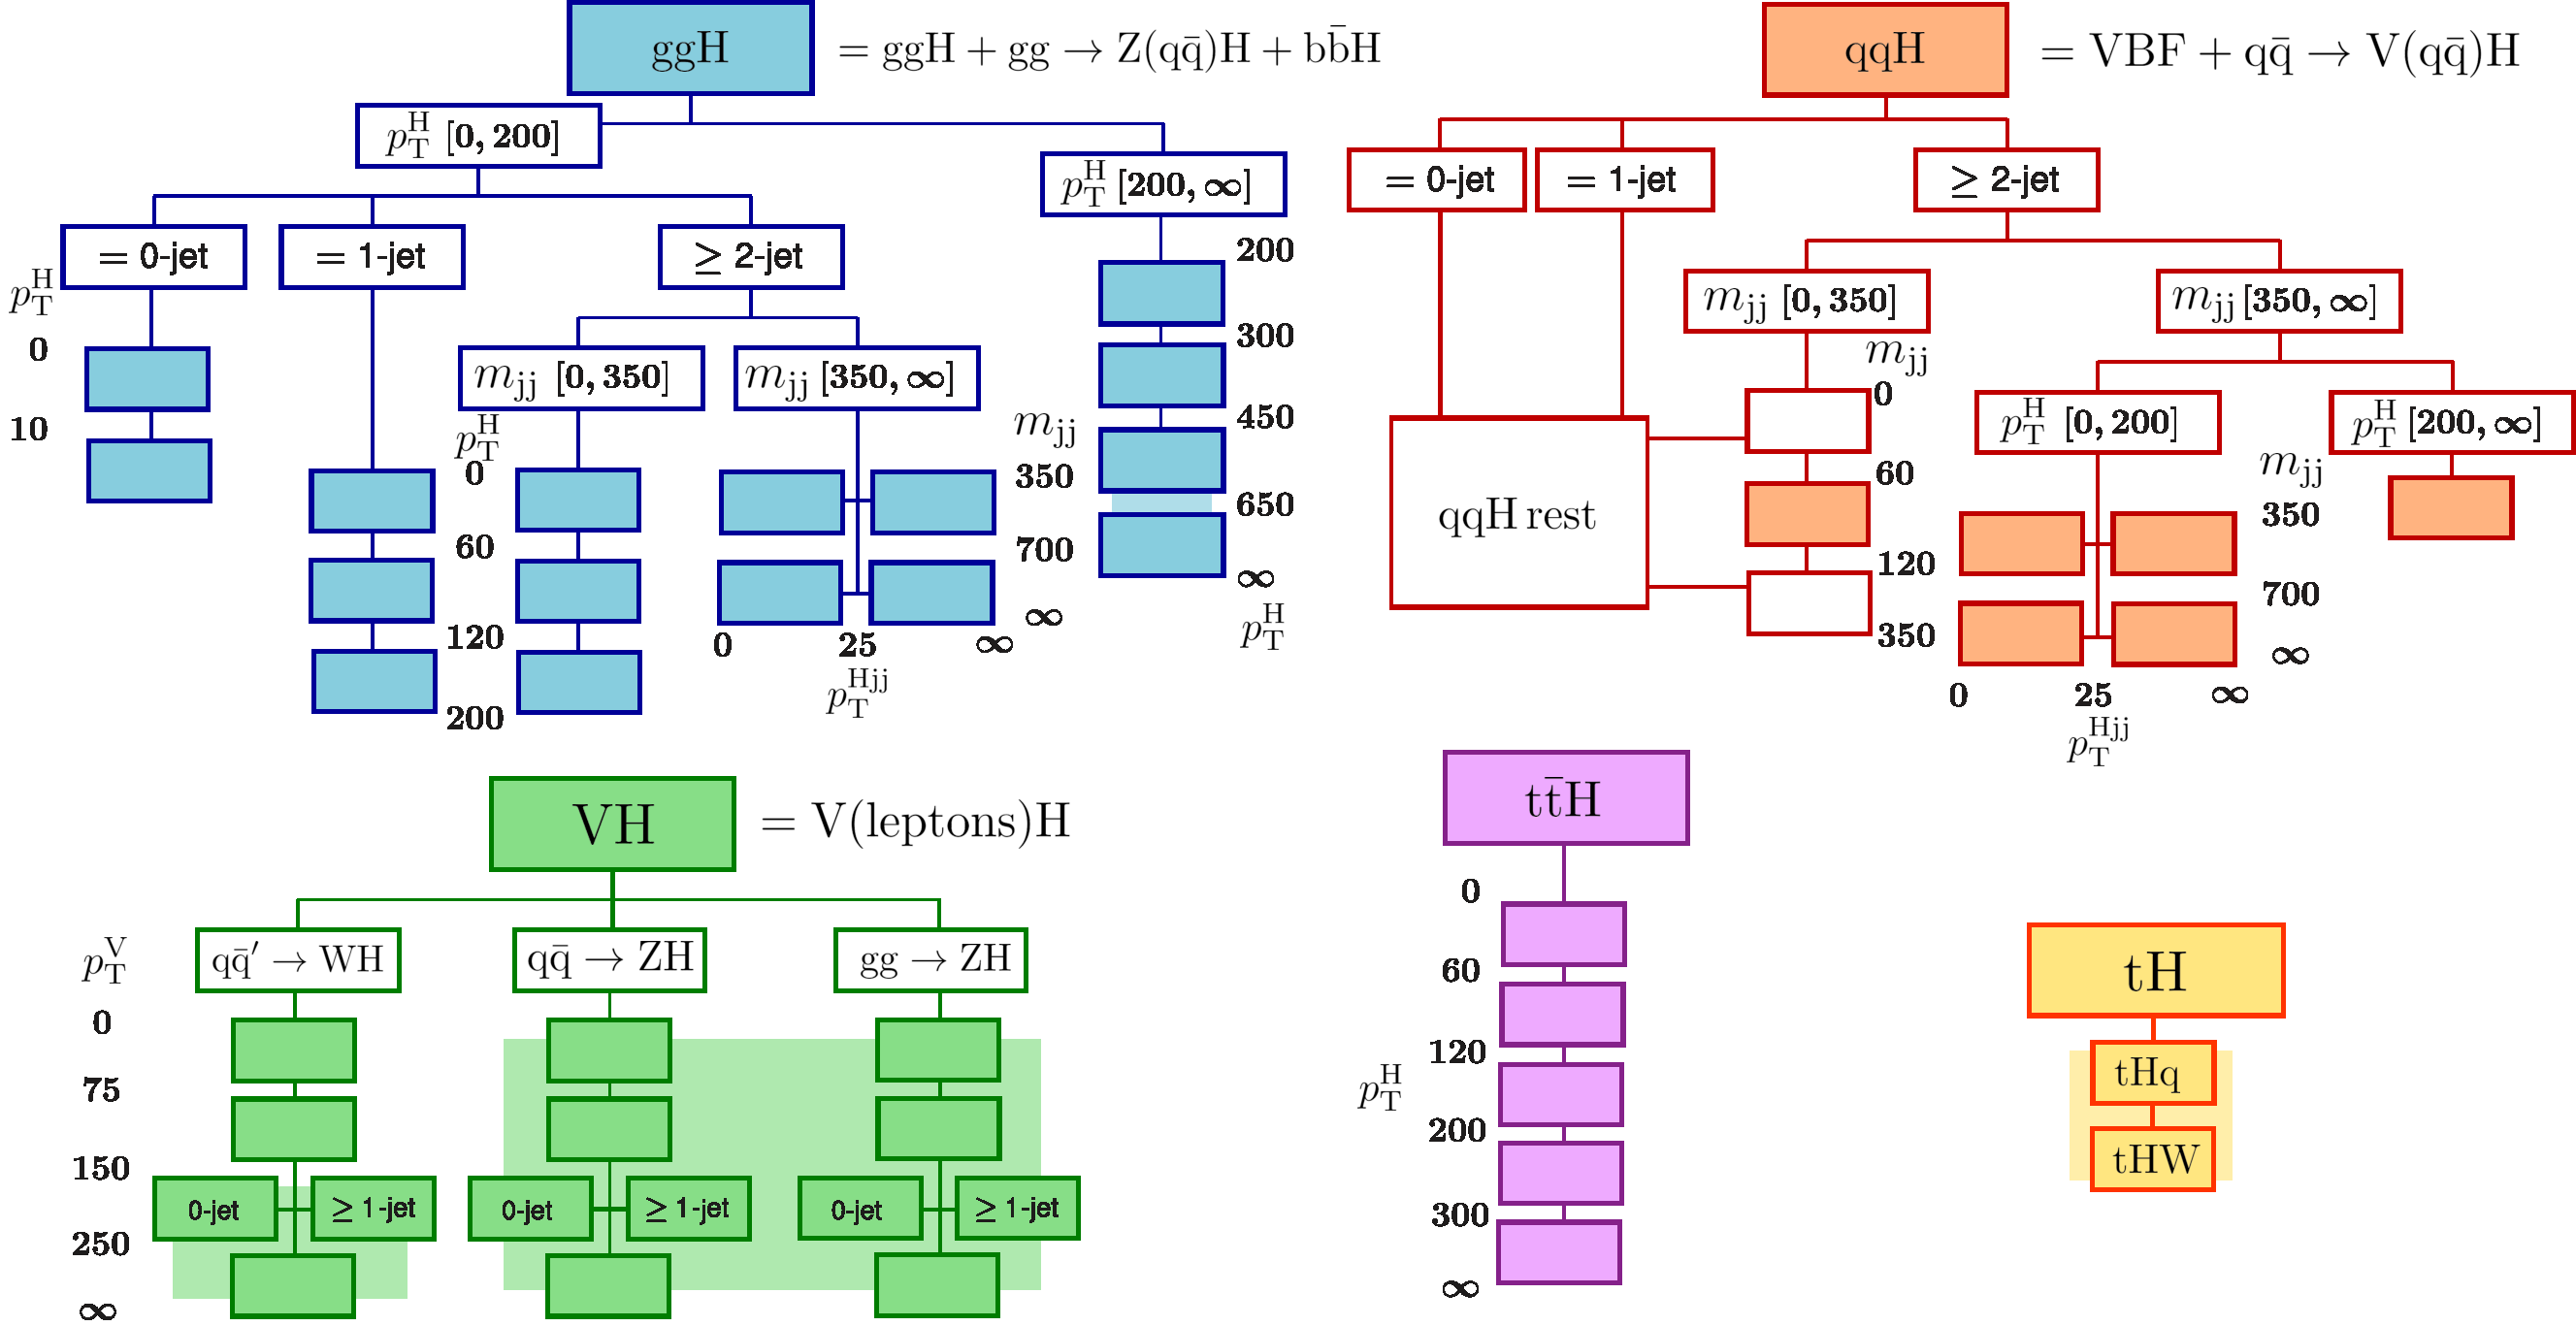
\includegraphics[width=1\linewidth]{Figures/theory/allSTXSbins.pdf}
  \caption[STXS stage 1.2 binning scheme]
  {
    Schematic of the full STXS stage 1.2 binning scheme, adapted from Ref.~\cite{deFlorian:2016spz}. This is defined for events with $|y_H|<2.5$. The solid boxes represent each STXS stage 1.2 bin. The units of $\ptH$, $\mgg$, $\ptHjj$, and $\ptV$ are in GeV. The shaded regions indicate the STXS bins which are divided at stage 1.2, but are not measured independently in the \Hgg analysis described in chapters~\ref{chap:hgg_overview}--\ref{chap:hgg_results}.
  }
  \label{fig:stxs_schematic}
\end{figure}

There are many advantages to cross section measurements in the STXS framework. Firstly, splitting the phase space into different kinematic bins systematically reduces the theory dependence of the measurements, in the sense that we no longer rely on the SM to predict the relative compositions of two different physics processes (STXS bins). Reducing the theory dependence in this fashion makes the measurements easier to re-interpret, and also helps to preserve the usefulness of the measurements as they are less affected by future improvements to the theoretical predictions. Moreover, the splitting helps to isolate specific kinematic regions of phase space which are likely to be affected by BSM physics e.g. ggH production with high $p_T^H$. 

Measurements in the STXS framework differ from standard differential cross sections measurements as they do not include a fiducial region definition of the final state particles in the event, including the Higgs boson decay products. This ultimately permits the use of sophisticated analysis techniques to optimise the sensitivity to the cross sections, such as the application of machine learning algorithms for event classification (see Appendix~\ref{app:ML}). Additionally, by being agnostic to the Higgs boson decay, the STXS framework enables the smooth combination of measurements across different Higgs boson decay channels. 

Whilst the benefits listed above are numerous, it is important to keep in mind that STXS measurements rely on SM simulation to model the experimental acceptance of events from a given STXS bin. This assumption may break down in the presence of BSM physics, which can modify the event kinematics and subsequently the within-bin experimental acceptance. In particular, new physics affecting the final state kinematics of the Higgs boson decay goes unaccounted for in the STXS framework as there is no fiducial selection on the decay products. Consequently, BSM re-interpretations of STXS measurements must be approached with care.

The remainder of the section provides a description of the stage 1.2 binning scheme used in the \Hgg analysis of chapters~\ref{chap:hgg_overview}--\ref{chap:hgg_results} (Figure~\ref{fig:stxs_schematic}). Throughout, the units of GeV are removed in the STXS bin naming for brevity. All events require the absolute value of the Higgs boson rapidity, $|y_H|$, to be less than 2.5, as events with values above this threshold are typically outside of the experimental acceptance. The ggH production mode (blue) is split into bins according to the Higgs boson transverse momentum ($p_T^H$) and the number of jets\footnote{In the STXS event classification, jets are defined with the \textsc{Fastjet} package~\cite{Cacciari:2011ma} using the anti-$k_T$ algorithm with a distance parameter of 0.4~\cite{Cacciari:2008gp}. This is applied to the particle-level event constituents after parton showering and hadronisation. All jets are required to have a transverse momentum, $p_T^j>30$~GeV. More detail concerning the definition of jets in simulation is provided in section~\ref{sec:mc}.}. The boosted kinematic region with ${p_T^H>200}$~GeV is particularly sensitive to BSM physics appearing in the ggH loop. This region is further split according to additional $p_T^H$ boundaries, which are measured for the first time in this thesis. 

\begin{table}[htb!]
    \caption[ggH STXS bin definitions]{Definition of the ggH STXS bins. The product of the cross section times \Hgg branching fraction, $\sigma_{\rm{SM}}\mathcal{B}$, evaluated at $\sqrt{s}=13$~TeV and $m_H=125$~GeV, is given for each bin in the final column. Additionally, the fraction of the total production mode cross section from each STXS bin is shown. Events originating from ggZH production, in which the Z decays hadronically, are grouped with ggH in the STXS measurements, and are shown as a separate column in the table. The bbH production mode, whose $\sigma_{\rm{SM}}\mathcal{B}=1.054$~fb, is grouped together with the ggH 0J high $p_T^H$ bin. Unless stated otherwise, the STXS bins are defined for $|y_H|<2.5$. Events with $|y_H|>2.5$ are mostly outside of experimental acceptance, and therefore make a negligible contribution to the \Hgg analysis.}
    \label{tab:ggH_definitions}
    % \vspace{.5cm}
    \centering
    \scriptsize
    \renewcommand{\arraystretch}{1.2}
    \setlength{\tabcolsep}{3pt}
    \hspace*{-3cm}
    \begin{tabular}{l|cccc}
   \multirow{2}{*}{STXS bin} & \multirow{2}{*}{\begin{tabular}[c]{@{}c@{}}Definition\\ units of $\ptH$, $\mjj$ and $\ptHjj$ in GeV\end{tabular}} & \multicolumn{2}{c}{Fraction of cross section} & \multirow{2}{*}{$\sigma_{\text{SM}}\mathcal{B}$~(fb)} \\
    &  & ggH & gg $\rightarrow$ Z(q$\bar{\rm{q}}$)H &  \\ [\cmsTabSkip] \hline
   ggH forward & $|Y_H| > 2.5$ & 8.09\% & 2.73\% & 8.93 \\ [\cmsTabSkip]
   ggH 0J low $\ptH$ & Exactly 0 jets, $\ptH$~$<$~10 & 13.87\% & 0.01\% & 15.30 \\
   ggH 0J high $\ptH$ & Exactly 0 jets, 10~$<$~$\ptH$~$<$~200 & 39.40\% & 0.29\% & 43.45 \\ [\cmsTabSkip]
   ggH 1J low $\ptH$ & Exactly 1 jet, $\ptH$~$<$~60 & 14.77\% & 2.00\% & 16.29 \\
   ggH 1J med $\ptH$ & Exactly 1 jet, 60~$<$~$\ptH$~$<$~120 & 10.23\% & 5.34\% & 11.29 \\
   ggH 1J high $\ptH$ & Exactly 1 jet, 120~$<$~$\ptH$~$<$~200 & 1.82\% & 3.53\% & 2.01 \\  [\cmsTabSkip]
   ggH $\geq$2J low $\ptH$ & At least 2 jets, $\ptH$~$<$~60, $\mjj$~$<$~350 & 2.56\% & 5.74\% & 2.83 \\
   ggH $\geq$2J med $\ptH$ & At least 2 jets, 60~$<$~$\ptH$~$<$~120, $\mjj$~$<$~350 & 4.10\% & 19.63\% & 4.56 \\
   ggH $\geq$2J high $\ptH$ & At least 2 jets, 120~$<$~$\ptH$~$<$~200, $\mjj$~$<$~350 & 1.88\% & 29.55\% & 2.13 \\  [\cmsTabSkip]
   ggH BSM 200~$<$~$\ptH$~$<$~300 & No jet requirements, 200~$<$~$\ptH$~$<$~300 & 0.98\% & 13.93\% & 1.11 \\
   ggH BSM 300~$<$~$\ptH$~$<$~450 & No jet requirements, 300~$<$~$\ptH$~$<$~450 & 0.25\% & 3.86\% & 0.28 \\
   ggH BSM 450~$<$~$\ptH$~$<$~650 & No jet requirements, 450~$<$~$\ptH$~$<$~650 & 0.03\% & 0.77\% & 0.03 \\
   ggH BSM $\ptH$~$>$~650 & No jet requirements, $\ptH$~$>$~650 & 0.01\% & 0.20\% & 0.01 \\ [\cmsTabSkip]
   ggH VBF-like low $\mjj$ low $\ptHjj$ & \begin{tabular}[c]{@{}c@{}}At least 2 jets, $\ptH$~$<$~200,\\ 350~$<$~$\mjj$~$<$~700, $\ptHjj$~$<$~25\end{tabular} & 0.63\% & 1.14\% & 0.70 \\
   ggH VBF-like low $\mjj$ high $\ptHjj$ & \begin{tabular}[c]{@{}c@{}}At least 2 jets, $\ptH$~$<$~200,\\ 350~$<$~$\mjj$~$<$~700, $\ptHjj$~$>$~25\end{tabular} & 0.77\% & 8.06\% & 0.86 \\
   ggH VBF-like high $\mjj$ low $\ptHjj$ & \begin{tabular}[c]{@{}c@{}}At least 2 jets, $\ptH$~$<$~200,\\ $\mjj$~$>$~700, $\ptHjj$~$<$~25\end{tabular} & 0.28\% & 0.36\% & 0.31 \\
   ggH VBF-like high $\mjj$ high $\ptHjj$ & \begin{tabular}[c]{@{}c@{}}At least 2 jets, $\ptH$~$<$~200,\\ $\mjj$~$>$~700, $\ptHjj$~$>$~25\end{tabular} & 0.32\% & 2.85\% & 0.36 \\
\end{tabular}
    \hspace*{-3cm}
\end{table}

Additionally, the ggH binning scheme defines a VBF-like region with high dijet invariant mass ($m_{jj}$). This VBF-like region is split into four bins according to $m_{jj}$ and the transverse momentum of the Higgs boson plus dijet system ($p_T^{Hjj}$). For the purpose of the \Hgg analysis, events originating from bbH production and ggZH production in which the associated Z boson decays hadronically, are grouped with ggH events. This choice is made since the current available data set is not sensitive to the independent measurements of these rarer production modes. The SM predicted cross section breakdown for the ggH STXS bins is given in Table~\ref{tab:ggH_definitions}. These values are calculated by classifying events in SM simulation, as described in section~\ref{sec:hgg_simulation}. The final column in the table lists the product of the cross section times \Hgg branching fraction, $\sigma_{\rm{SM}}\mathcal{B}$, for each bin. Ultimately, these are the observables that the \Hgg analysis aims to measure, and by comparing to the SM predictions it is possible to constrain (or more optimistically infer) the presence of new physics.

% \begin{table}[htb!]
%     \caption[ggH STXS bin definitions]{Definition of the ggH STXS bins. The product of the cross section times \Hgg branching fraction, $\sigma_{\rm{SM}}\mathcal{B}$, evaluated at $\sqrt{s}=13$~TeV and $m_H=125$~GeV, is given for each bin in the final column. Additionally, the fraction of the total production mode cross section from each STXS bin is shown. Events originating from ggZH production, in which the Z decays hadronically, are grouped with ggH in the STXS measurements, and are shown as a separate column in the table. The bbH production mode, whose $\sigma_{\rm{SM}}\mathcal{B}=1.054$~fb, is grouped together with the ggH 0J high $p_T^H$ bin. Unless stated otherwise, the STXS bins are defined for $|y_H|<2.5$. Events with $|y_H|>2.5$ are mostly outside of experimental acceptance, and therefore make a negligible contribution to the \Hgg analysis.}
%     \label{tab:ggH_definitions}
%     % \vspace{.5cm}
%     \centering
%     \scriptsize
%     \renewcommand{\arraystretch}{1.2}
%     \setlength{\tabcolsep}{3pt}
%     \hspace*{-3cm}
%     \begin{tabular}{l|cccc}
   \multirow{2}{*}{STXS bin} & \multirow{2}{*}{\begin{tabular}[c]{@{}c@{}}Definition\\ units of $\ptH$, $\mjj$ and $\ptHjj$ in GeV\end{tabular}} & \multicolumn{2}{c}{Fraction of cross section} & \multirow{2}{*}{$\sigma_{\text{SM}}\mathcal{B}$~(fb)} \\
    &  & ggH & gg $\rightarrow$ Z(q$\bar{\rm{q}}$)H &  \\ [\cmsTabSkip] \hline
   ggH forward & $|Y_H| > 2.5$ & 8.09\% & 2.73\% & 8.93 \\ [\cmsTabSkip]
   ggH 0J low $\ptH$ & Exactly 0 jets, $\ptH$~$<$~10 & 13.87\% & 0.01\% & 15.30 \\
   ggH 0J high $\ptH$ & Exactly 0 jets, 10~$<$~$\ptH$~$<$~200 & 39.40\% & 0.29\% & 43.45 \\ [\cmsTabSkip]
   ggH 1J low $\ptH$ & Exactly 1 jet, $\ptH$~$<$~60 & 14.77\% & 2.00\% & 16.29 \\
   ggH 1J med $\ptH$ & Exactly 1 jet, 60~$<$~$\ptH$~$<$~120 & 10.23\% & 5.34\% & 11.29 \\
   ggH 1J high $\ptH$ & Exactly 1 jet, 120~$<$~$\ptH$~$<$~200 & 1.82\% & 3.53\% & 2.01 \\  [\cmsTabSkip]
   ggH $\geq$2J low $\ptH$ & At least 2 jets, $\ptH$~$<$~60, $\mjj$~$<$~350 & 2.56\% & 5.74\% & 2.83 \\
   ggH $\geq$2J med $\ptH$ & At least 2 jets, 60~$<$~$\ptH$~$<$~120, $\mjj$~$<$~350 & 4.10\% & 19.63\% & 4.56 \\
   ggH $\geq$2J high $\ptH$ & At least 2 jets, 120~$<$~$\ptH$~$<$~200, $\mjj$~$<$~350 & 1.88\% & 29.55\% & 2.13 \\  [\cmsTabSkip]
   ggH BSM 200~$<$~$\ptH$~$<$~300 & No jet requirements, 200~$<$~$\ptH$~$<$~300 & 0.98\% & 13.93\% & 1.11 \\
   ggH BSM 300~$<$~$\ptH$~$<$~450 & No jet requirements, 300~$<$~$\ptH$~$<$~450 & 0.25\% & 3.86\% & 0.28 \\
   ggH BSM 450~$<$~$\ptH$~$<$~650 & No jet requirements, 450~$<$~$\ptH$~$<$~650 & 0.03\% & 0.77\% & 0.03 \\
   ggH BSM $\ptH$~$>$~650 & No jet requirements, $\ptH$~$>$~650 & 0.01\% & 0.20\% & 0.01 \\ [\cmsTabSkip]
   ggH VBF-like low $\mjj$ low $\ptHjj$ & \begin{tabular}[c]{@{}c@{}}At least 2 jets, $\ptH$~$<$~200,\\ 350~$<$~$\mjj$~$<$~700, $\ptHjj$~$<$~25\end{tabular} & 0.63\% & 1.14\% & 0.70 \\
   ggH VBF-like low $\mjj$ high $\ptHjj$ & \begin{tabular}[c]{@{}c@{}}At least 2 jets, $\ptH$~$<$~200,\\ 350~$<$~$\mjj$~$<$~700, $\ptHjj$~$>$~25\end{tabular} & 0.77\% & 8.06\% & 0.86 \\
   ggH VBF-like high $\mjj$ low $\ptHjj$ & \begin{tabular}[c]{@{}c@{}}At least 2 jets, $\ptH$~$<$~200,\\ $\mjj$~$>$~700, $\ptHjj$~$<$~25\end{tabular} & 0.28\% & 0.36\% & 0.31 \\
   ggH VBF-like high $\mjj$ high $\ptHjj$ & \begin{tabular}[c]{@{}c@{}}At least 2 jets, $\ptH$~$<$~200,\\ $\mjj$~$>$~700, $\ptHjj$~$>$~25\end{tabular} & 0.32\% & 2.85\% & 0.36 \\
\end{tabular}
%     \hspace*{-3cm}
% \end{table}

The electroweak qqH production scheme (orange) considers both VBF production and VH production in which the vector boson decays hadronically. This reflects the fact that VBF and VH hadronic production are the t+u-channel and s-channel diagrams, respectively, of the same physics process: qq$\rightarrow$Hqq, and therefore cannot be distinguished at higher orders. The kinematic bins are defined according to the number of jets, $\ptH$, $\mjj$, and $\ptHjj$, in the attempt to isolate different topologies of qqH events. Firstly, the bin with the dijet invariant mass window $60<\mjj<120$~GeV specifically targets VH hadronic production. Akin to the ggH scheme, events with a VBF-like topology are defined by the region with $\mjj>350$~GeV, which is further split into four bins according to boundaries in \mjj and \ptHjj. Finally, the BSM-sensitive region with a boosted Higgs boson is defined by a single bin with $p_T^H>200$~GeV. The four STXS bins which define the qqH rest region (see Figure~\ref{fig:stxs_schematic}) are not explicitly probed in the \Hgg analysis. Table~\ref{tab:qqH_definitions} provides the SM predicted cross section breakdown for the qqH STXS bins.

\begin{table}[htb!]
    \caption[qqH STXS bin definitions]{Definition of the qqH STXS bins. The product of the cross section times \Hgg branching fraction, $\sigma_{\rm{SM}}\mathcal{B}$, evaluated at $\sqrt{s}=13$~TeV and $m_H=125$~GeV, is given for each bin in the final column. Additionally, the fraction of the total production mode cross section from each STXS bin is shown. Unless stated otherwise, the STXS bins are defined for $|y_H|<2.5$. Events with $|y_H|>2.5$ are mostly outside of experimental acceptance, and therefore make a negligible contribution to the \Hgg analysis.}
    \label{tab:qqH_definitions}
    % \vspace{.5cm}
    \centering
    \scriptsize
    \renewcommand{\arraystretch}{1.2}
    \setlength{\tabcolsep}{3pt}
    \hspace*{-3cm}
    \begin{tabular}{l|c|ccc|c}
   \multirow{2}{*}{STXS bin} & \multirow{2}{*}{\begin{tabular}[c]{@{}c@{}}Definition\\ units of $p_T^H$, $\mjj$ and $\ptHjj$ in GeV\end{tabular}} & \multicolumn{3}{c|}{Fraction of total} & \multirow{2}{*}{$\sigma_{\text{SM}}\mathcal{B}$~[fb]} \\ 
    &  & VBF & qq$\rightarrow$W(qq)H & qq$\rightarrow$Z(qq)H &  \\ [\cmsTabSkip] \hline
   qqH forward & $|Y_H| > 2.5$ & 6.69\% & 12.57\% & 9.84\% & 0.98 \\ [\cmsTabSkip]
   %\multicolumn{6}{c}{$|Y_H| < 2.5$} \\ \hline
   qqH 0J & Exactly 0 jets & 6.95\% & 5.70\% & 3.73\% & 0.77 \\ 
   qqH 1J & Exactly 1 jet & 32.83\% & 31.13\% & 25.03\% & 3.82 \\ 
   qqH $\mjj$~$<$~60 & At least 2 jets, $\mjj$~$<$~60 & 1.36\% & 3.58\% & 2.72\% & 0.23 \\ 
   qqH VH-like & At least 2 jets, 60~$<$~$\mjj$~$<$~120 & 2.40\% & 29.43\% & 28.94\% & 1.23 \\ 
   qqH 120~$<$~$\mjj$~$<$~350 & At least 2 jets, 120~$<$~$\mjj$~$<$~350 & 12.34\% & 13.92\% & 12.59\% & 1.53 \\ [\cmsTabSkip]
   qqH VBF-like low $\mjj$ low $\ptHjj$ & \begin{tabular}[c]{@{}c@{}}At least 2 jets, $\ptH$~$<$~200,\\ 350~$<$~$\mjj$~$<$~700, $\ptHjj$~$<$~25\end{tabular} & 10.26\% & 0.44\% & 0.35\% & 0.90 \\ 
   qqH VBF-like low $\mjj$ high $\ptHjj$ & \begin{tabular}[c]{@{}c@{}}At least 2 jets, $\ptH$~$<$~200,\\ 350~$<$~$\mjj$~$<$~700, $\ptHjj$~$>$~25\end{tabular} & 3.85\% & 1.86\% & 1.74\% & 0.39 \\ 
   qqH VBF-like high $\mjj$ low $\ptHjj$ & \begin{tabular}[c]{@{}c@{}}At least 2 jets, $\ptH$~$<$~200,\\ $\mjj$~$>$~700, $\ptHjj$~$<$~25\end{tabular} & 15.09\% & 0.09\% & 0.08\% & 1.30 \\ 
   qqH VBF-like high $\mjj$ high $\ptHjj$ & \begin{tabular}[c]{@{}c@{}}At least 2 jets, $\ptH$~$<$~200,\\ $\mjj$~$>$~700, $\ptHjj$~$>$~25\end{tabular} & 4.25\% & 0.40\% & 0.39\% & 0.38 \\ 
   qqH BSM & At least 2 jets, $\mjj$~$>$~350, $p_T^H$~$>$~200 & 3.98\% & 0.88\% & 0.71\% & 0.37 \\ 
\end{tabular}

    \hspace*{-3cm}
\end{table}

Events produced via the VH and ggZH production modes, in which the vector boson decays leptonically are categorised according to the VH leptonic binning scheme (green). Three equivalent regions are defined for WH, ZH and ggZH production, with kinematic boundaries in the transverse momentum of the vector boson ($\ptV$) and the number of jets. The SM predicted cross section breakdown for the VH leptonic STXS bins is listed in Table~\ref{tab:vh_definitions}.

\begin{table}[htb!]
    \caption[VH leptonic STXS bin definitions]{Definition of the VH leptonic STXS bins. The product of the cross section times \Hgg branching fraction, $\sigma_{\rm{SM}}\mathcal{B}$, evaluated at $\sqrt{s}=13$~TeV and $m_H=125$~GeV, is given for each bin in the final column. Additionally, the fraction of the total production mode cross section from each STXS bin is shown. Unless stated otherwise, the STXS bins are defined for $|y_H|<2.5$. Events with $|y_H|>2.5$ are mostly outside of experimental acceptance, and therefore make a negligible contribution to the \Hgg analysis.}
    \label{tab:vh_definitions}
    % \vspace{.5cm}
    \centering
    \scriptsize
    \renewcommand{\arraystretch}{1.2}
    \setlength{\tabcolsep}{5pt}
    \hspace*{-2cm}
    \begin{tabular}{l|ccccc}
    \hline
   \multirow{2}{*}{STXS bin} & \multirow{2}{*}{\begin{tabular}[c]{@{}c@{}}Definition\\ units of $\ptV$ in GeV\end{tabular}} & \multicolumn{3}{c}{Fraction of cross section} & \multirow{2}{*}{$\sigma_{\text{SM}}\mathcal{B}$~(fb)} \\
    &  & q$\bar{\rm{q}}'\rightarrow$WH & q$\bar{\rm{q}}'\rightarrow$ZH & gg$\rightarrow$ZH &  \\ [\cmsTabSkip] \hline
   WH lep forward& \multirow{3}{*}{$|Y_H| > 2.5$}& 12.13\%& -& -& 0.123 \\
   ZH lep forward& & -& 11.21\%& -& 0.058 \\
   ggZH lep forward& & -& -& 2.71\%& 0.002 \\ [\cmsTabSkip]
   %\multicolumn{6}{c}{$|Y_H| < 2.5$} \\ \hline
   WH lep $\ptV$~$<$~75 & No jet requirements, $\ptV$~$<$~75 & 46.55\% & - & - & 0.473 \\
   WH lep 75~$<$~$\ptV$~$<$~150 & No jet requirements, 75~$<$~$\ptV$~$<$~150 & 29.30\% & - & - & 0.298 \\
   WH lep 0J 150~$<$~$\ptV$~$<$~250 & Exactly 0 jets, 150~$<$~$\ptV$~$<$~250 & 5.10\% & - & - & 0.052 \\
   WH lep $\geq$1J 150~$<$~$\ptV$~$<$~250 & At least 1 jet, 150~$<$~$\ptV$~$<$~250 & 3.97\% & - & - & 0.040 \\
   WH lep $\ptV$~$>$~250 & No jet requirements, $\ptV$~$>$~250 & 2.95\% & - & - & 0.030 \\ [\cmsTabSkip]
   ZH lep $\ptV$~$<$~75 & No jet requirements, $\ptV$~$<$~75 & - & 45.65\% & - & 0.237 \\
   ZH lep 75~$<$~$\ptV$~$<$~150 & No jet requirements, 75~$<$~$\ptV$~$<$~150 & - & 30.70\% & - & 0.160 \\
   ZH lep 0J 150~$<$~$\ptV$~$<$~250 & Exactly 0 jets, 150~$<$~$\ptV$~$<$~250 & - & 5.16\% & - & 0.027 \\
   ZH lep $\geq$1J 150~$<$~$\ptV$~$<$~250 & At least 1 jet, 150~$<$~$\ptV$~$<$~250 & - & 4.27\% & - & 0.022 \\
   ZH lep $\ptV$~$>$~250 & No jet requirements, $\ptV$~$>$~250 & - & 3.01\% & - & 0.016 \\ [\cmsTabSkip]
   ggZH lep $\ptV$~$<$~75 & No jet requirements, $\ptV$~$<$~75 & - & - & 15.96\% & 0.013 \\
   ggZH lep 75~$<$~$\ptV$~$<$~150 & No jet requirements, 75~$<$~$\ptV$~$<$~150 & - & - & 43.32\% & 0.036 \\
   ggZH lep 0J 150~$<$~$\ptV$~$<$~250 & Exactly 0 jets, 150~$<$~$\ptV$~$<$~250 & - & - & 9.08\% & 0.008 \\
   ggZH lep $\geq$1J 150~$<$~$\ptV$~$<$~250 & At least 1 jet, 150~$<$~$\ptV$~$<$~250 & - & - & 20.49\% & 0.017 \\
   ggZH lep $\ptV$~$>$~250 & No jet requirements, $\ptV$~$>$~250 & - & - & 8.45\% & 0.007 \\
   \hline
\end{tabular}

    \hspace*{-2cm}
\end{table}

The ttH production mode (pink) is split according to four boundaries in $\ptH$. This splitting was first introduced at stage 1.2, and consequently the \Hgg analysis documented here is the first to measure ttH production in different kinematic regions. Finally, there is an additional tH production STXS bin (yellow), which includes contributions from both the tHq and tHW production modes. This thesis also includes the first explicit measurement of tH production cross section in the \Hgg decay channel. Table~\ref{tab:top_definitions} gives the SM predicted cross section breakdown for the top-associated STXS bins.


\begin{table}[htb!]
    \caption[Top-associated STXS bin definitions]{Definition of the top-associated STXS bins. The product of the cross section times \Hgg branching fraction, $\sigma_{\rm{SM}}\mathcal{B}$, evaluated at $\sqrt{s}=13$~TeV and $m_H=125$~GeV, is given for each bin in the final column. Additionally, the fraction of the total production mode cross section from each STXS bin is shown. Unless stated otherwise, the STXS bins are defined for $|y_H|<2.5$. Events with $|y_H|>2.5$ are mostly outside of experimental acceptance, and therefore make a negligible contribution to the \Hgg analysis.}
    \label{tab:top_definitions}
    % \vspace{.5cm}
    \centering
    \scriptsize
    \renewcommand{\arraystretch}{1.5}
    \setlength{\tabcolsep}{5pt}
    % \hspace*{-5cm}
    \begin{tabular}{l|c|cccc|c}
   \multirow{2}{*}{STXS region} & \multirow{2}{*}{\begin{tabular}[c]{@{}c@{}}Definition\\ units of $\ptH$ in GeV\end{tabular}} & \multicolumn{4}{c|}{Fraction of total} & \multirow{2}{*}{$\sigma_{\text{SM}}\mathcal{B}$~[fb]} \\ 
    &  & ttH & tHq & tHW & bbH &  \\ [\cmsTabSkip] \hline
   ttH forward& \multirow{3}{*}{$|Y_H| > 2.5$}& 1.35\%& -& -& -& 0.016 \\  
   tH forward& & -& 2.79\%& 1.06\%& -& 0.005 \\  
   bbH forward& & -& -& -& 4.87\%& 0.054 \\ [\cmsTabSkip] 
   %\multicolumn{7}{c}{$|Y_H| < 2.5$} \\ \hline
   ttH $\ptH$~$<$~60 & No jet requirements, $\ptH$~$<$~60 & 22.42\% & - & - & - & 0.259 \\ 
   ttH 60~$<$~$\ptH$~$<$~120 & No jet requirements, 60~$<$~$\ptH$~$<$~120 & 34.61\% & - & - & - & 0.400 \\ 
   ttH 120~$<$~$\ptH$~$<$~200 & No jet requirements, 120~$<$~$\ptH$~$<$~200 & 25.60\% & - & - & - & 0.296 \\ 
   ttH 200~$<$~$\ptH$~$<$~300 & No jet requirements, 200~$<$~$\ptH$~$<$~300 & 10.72\% & - & - & - & 0.124 \\ 
   ttH $\ptH$~$>$~300 & No jet requirements, $\ptH$~$>$~300 & 5.31\% & - & - & - & 0.061 \\ [\cmsTabSkip] 
   tH & No additional requirements & - & 97.21\% & 98.94\% & - & 0.204 \\ 
   bbH & No additional requirements & - & - & - & 95.13\% & 1.054 \\ 
\end{tabular}

    % \hspace*{-5cm}
\end{table}

\FloatBarrier

\section{Effective field theory}\label{sec:theory_eft}
The chapter concludes with an introduction to effective field theory (EFT), which is later applied in a BSM interpretation of STXS measurements in chapter~\ref{chap:eft}. EFT is by no means a new concept in particle physics. In 1933, Enrico Fermi formulated a low energy description of nuclear $\beta$-decay as a four-fermion contact interaction (an interaction which occurs at a single point in space-time) between a neutron, electron, (anti)-neutrino, and a proton~\cite{Fermi:1933jpa}. This is expressed by the matrix element\footnote{This expression includes a modification of the original Fermi theory to incorporate the effects of parity violation, observed experimentally by Wu \textit{et. al.} in 1957~\cite{PhysRev.105.1413}.},

\begin{equation}\label{eq:fermi_theory}
    \mathcal{M}_{i \rightarrow f} = \frac{1}{\sqrt{2}}G_F \eta_{\mu\nu} (\bar{\psi}_3 \gamma^\mu(1-\gamma^5) \psi_1)(\bar{\psi}_4 \gamma^\nu(1-\gamma^5) \psi_2),
\end{equation}

\noindent
where $G_F$ governs the strength of the contact interaction, and is referred to as the Fermi constant. It is now known that this process is described by the weak interaction, and occurs via the exchange of a W boson. This has a corresponding matrix element,

\begin{equation}
    \mathcal{M}_{i \rightarrow f} = -\Big( \frac{1}{2\sqrt{2}}g\bar{\psi}_3 \gamma^\mu(1-\gamma^5) \psi_1 \Big) \cdot \Big( \frac{\eta_{\mu\nu}-q_{\mu}q_\nu/m_W^2}{q^2-m_W^2} \Big) \cdot \Big( \frac{1}{2\sqrt{2}}g\bar{\psi}_4 \gamma^\nu(1-\gamma^5) \psi_2 \Big).
\end{equation}

\noindent
In the low energy ($q^2 \ll m_W^2$) limit, this simply reduces to the matrix element from Fermi's theory (equation~\ref{eq:fermi_theory}). In other words, Fermi's theory provides a low-energy \textit{effective field theory} of the weak interaction. Moreover, we can \textit{match} the contact interaction strength, $G_F$, to the parameters of the complete high energy theory:

\begin{equation}
    \frac{G_F}{\sqrt{2}} = \frac{g^2}{8m_W^2},
\end{equation}

\noindent
where $g$ is the weak interaction coupling strength, and $m_W$ is the mass of the W boson. Hence, by measuring $G_F$ experimentally, it is possible to infer some knowledge concerning the high energy theory (in this case being the weak interaction). The application of EFT in the weak interaction is shown diagrammatically in Figure~\ref{fig:fermi_theory}.

\begin{figure}[htb!]
  \centering
  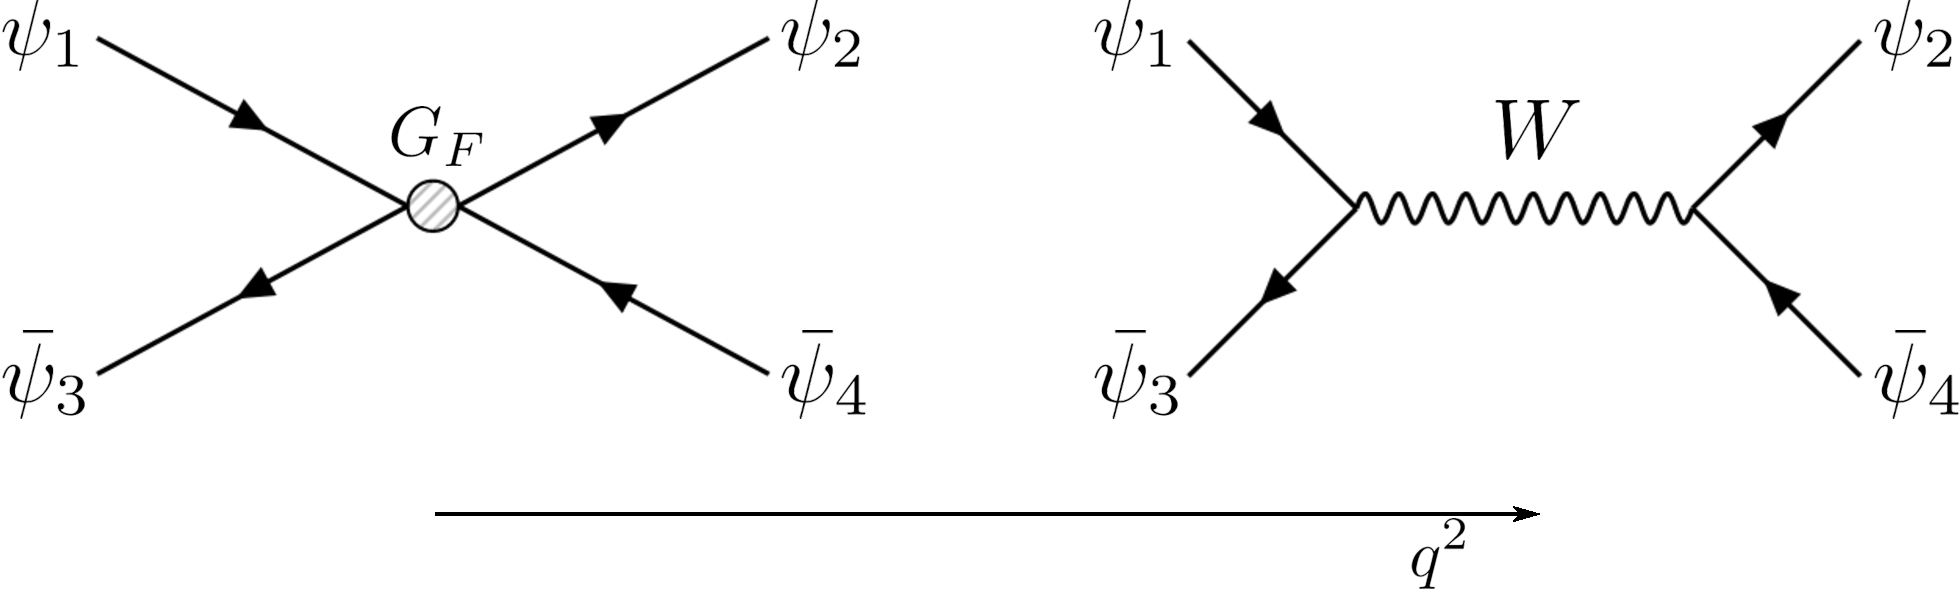
\includegraphics[width=.8\linewidth]{Figures/theory/fermi_theory.pdf}
  \caption[Fermi's theory of the weak interaction]
  {
    Fermi's theory, which models the weak interaction at low energies ($q^2 \ll m_W^2$) as a contact interaction between four fermions (left). At energies approaching $m_W$, the exchange of the W boson is required to correctly describe the interaction (right).
  }
  \label{fig:fermi_theory}
\end{figure}

EFT can be used to extend the SM Lagrangian to provide a (almost) model independent approach to search for BSM physics~\cite{Brivio:2017vri}. First, we assume that any new BSM states reside at an energy scale, $\Lambda$, far beyond the electroweak scale: $\Lambda \gg v$. This allows us to replace the non-local interactions involving the exchange of new particles, by contact interactions between the SM fields. In essence, the EFT describes the effect of the UV (ultraviolet) short-distance BSM physics on the IR (infrared) long-distance SM physics, without the need to construct a fully consistent BSM theory. Albeit, the validity of this approach is restricted to energies below the new physics mass scale, $\Lambda$.

The contact interactions are expressed mathematically as higher dimensional operators of the SM fields. The action of a Lagrangian, $S=\int {\rm{d}}^4x\,\mathcal{L}$, is a dimensionless quantity. Consequently, the operators in the SM Lagrangian, $\mathcal{L}_{\rm{SM}}$, must be of (energy) dimension-4\footnote{$[{\rm{d}}^4x]=4$ in terms of $x$, and $[x]=[E]^{-1}$, where $E$ is energy.}, and from this we infer the dimension of the SM fields to be the values listed in Table~\ref{tab:dimension}. The EFT Lagrangian, $\mathcal{L}_{\rm{EFT}}$, extends $\mathcal{L}_{\rm{SM}}$ with higher-dimensional operators according to,

\begin{equation}\label{eq:eft_expansion}
    \mathcal{L}_{\rm{EFT}} = \mathcal{L}^{\rm{(4)}}_{\rm{SM}} + \mathcal{L}^{\rm{(5)}} + \mathcal{L}^{\rm{(6)}} + \mathcal{L}^{\rm{(7)}} + \mathcal{L}^{\rm{(8)}} + {\rm{...}} \, ,
\end{equation}

\noindent
where the higher-order terms are of the form,

\begin{equation}\label{eq:eft_term}
    \mathcal{L}^{\rm{(d)}} = \sum^{N^{\rm{(d)}}}_{p=1} \frac{w^{\rm{(d)}}_p}{\Lambda^{{\rm{d}}-4}} \mathcal{O}^{\rm{(d)}}_p.
\end{equation}

\noindent
Here, $\mathcal{O}^{\rm{(d)}}_p$ is a dimension d operator constructed from the SM fields (Table~\ref{tab:dimension}), and $w^{\rm{(d)}}_p$ is the corresponding \textit{Wilson coefficient}. These Wilson coefficients embed the influence of the UV BSM physics on the IR operator, $\mathcal{O}^{\rm{(d)}}_p$, such that a deviation from zero in $w^{\rm{(d)}}_p$ implies the existence of new physics. In the context of Fermi's theory, the operator ${\mathcal{O}=\eta_{\mu\nu} (\bar{\psi}_3 \gamma^\mu(1-\gamma^5) \psi_1)(\bar{\psi}_4 \gamma^\nu(1-\gamma^5) \psi_2)}$ describes the four-fermion contact interaction, whilst $G_F$ is related to the corresponding Wilson coefficient, encoding the strength of the (high-energy) weak interaction. In summary, by measuring the set of $w^{\rm{(d)}}_p$ coefficients in experiment, we can infer not only the strength of new physics interactions, but also the relevant processes which are affected.

\begin{table}[htb]
    \caption[Dimension of the SM Lagrangian terms]{The dimension of the SM Lagrangian terms.}
    \label{tab:dimension}
    % \vspace{.5cm}
    \centering
    \footnotesize
    \setlength{\tabcolsep}{8pt}
    \renewcommand{\arraystretch}{1.2}
    \begin{tabular}{l|c}
        Term & Dimension \\ \hline
        Field strength tensors: $G^a_{\mu\nu}$, $W^i_{\mu\nu}$, $B_{\mu\nu}$ & 2 \\
        Derivative: $\partial_\mu$ & 1 \\
        Gauge fields: $G^a_\mu$, $W^i_\mu$, $B_\mu$ & 1 \\
        Covariant derivative: $D_\mu$ & 1 \\
        Higgs field: $H$ & 1 \\
        Higgs vacuum expectation value: $v$ & 1 \\
        Fermion fields: $\psi$ & 3/2 \\
        All couplings: $\lambda$, $g$, $\lambda_i$ etc & 0 \\
    \end{tabular}
\end{table}

In order to keep the action dimensionless, the higher order contributions enter with an energy scale suppression of $\Lambda^{-({\rm{d}}-4)}$. For example, the dimension-6 terms and dimension-8 terms are suppressed by factor $\Lambda^{-2}$ and $\Lambda^{-4}$, respectively. As a consequence, lower dimensional operators have a larger impact on physics observables. The total number of operators at dimension d is expressed as $N^{\rm{(d)}}$. At dimension-6 there are 2499 CP-even operators, which are typically reduced to a manageable number by assuming certain flavour symmetries in the model e.g. with minimal flavour violation, the number of independent operators reduces to 59~\cite{Alonso:2013hga}. This feature of EFT becomes increasingly problematic at higher dimensions, such that at dimension-8 there are 44,807 independent operators that enter the EFT Lagrangian~\cite{Murphy:2020rsh}. Ultimately, when measuring EFT parameters in experiment, we typically consider only a subset of (the most relevant) operators.

Dimension-5 operators violate lepton number conservation~\cite{Weinberg:1979sa}, whilst all other odd dimension operators violate the conservation of baryon number minus lepton number~\cite{deGouvea:2014lva}. So far, all LHC measurements suggest these approximate symmetries are conserved, and therefore odd dimension operators are not considered in this thesis. Moreover, due to the energy scale suppression, all terms of dimension-8 and higher are ignored, leaving only dimension-6 contributions to the Lagrangian,

\begin{equation}\label{eq:eft_expansion}
    \mathcal{L}_{\rm{EFT}} = \mathcal{L}^{\rm{(4)}}_{\rm{SM}} + \mathcal{L}^{\rm{(6)}}.
\end{equation}

Let's introduce a concrete example. In the SM, the Higgs field does not couple to the gluon field. Moving to dimension-6, it is possible to construct a gauge invariant operator of the form,
\begin{equation}
    \mathcal{O}^{\rm{(6)}}_G = |H|^2G^a_{\mu\nu}G^{a,\mu\nu}.
\end{equation}
\noindent
which describes the effective contact interaction between the Higgs and gluon fields (Figure~\ref{fig:eft_gluon}, right). The corresponding Wilson coefficient, $w^{\rm{(6)}}_G$, encodes the contribution from new physics in this interaction, such that a value different from zero would imply the existence of some new BSM state that couples to the Higgs and the gluon fields (Figure~\ref{fig:eft_gluon}, left). Approaching the problem in this way means we are agnostic to the specifics of the UV-complete BSM theory, or in other words, it enables a model-independent method to search for BSM physics. If required, the measurements of the Wilson coefficients can be systematically \textit{matched} to UV-complete BSM theories to place constraints on the particle masses and couplings of the theory. Further detail on this matching procedure, with specific examples, is provided in Ref.~\cite{Marzocca:2020jze}. 

\begin{figure}[htb!]
  \centering
  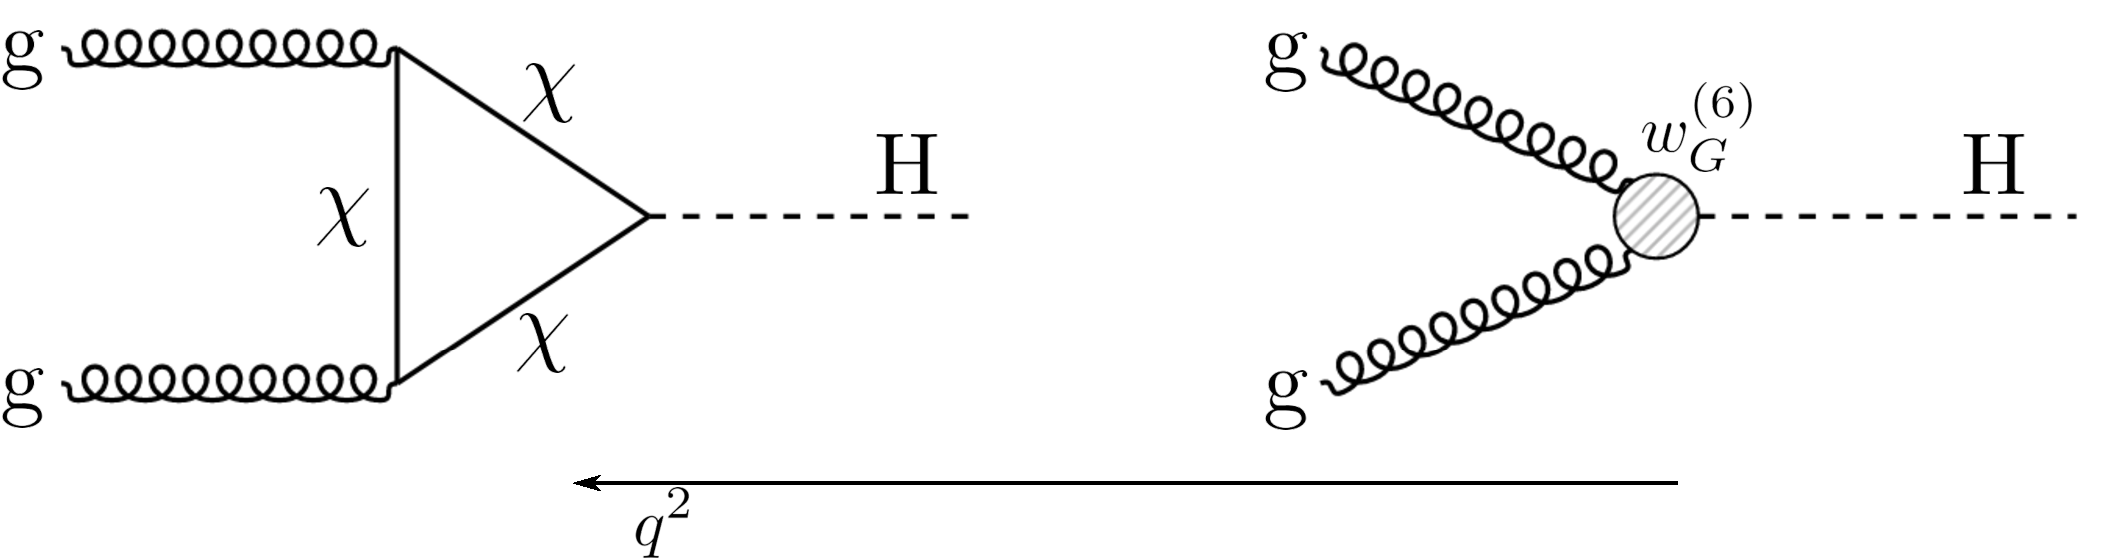
\includegraphics[width=.8\linewidth]{Figures/theory/og_operator.pdf}
  \caption[Higgs-gluon contact interaction]
  {
    Modelling BSM physics state, $\chi$, at low energy ($q^2\ll\Lambda^2$) with the dimension-6 contact interaction between the Higgs and gluon fields.
  }
  \label{fig:eft_gluon}
\end{figure}

The modified dynamics of the SM fields are derived by the applying the Euler-Lagrange equations to $\mathcal{L}_{\rm{EFT}}$. This provides a new set of Feynman rules, which subsequently describe how the additional contact interactions affect the experimentally measured observables: $\sigma$ and $\Gamma$. Crucially, the effects are not limited to the inclusive rates, but also modify the kinematic properties of the events. This makes STXS measurements an excellent candidate for probing EFT effects in the Higgs sector, as the additional kinematic information they provide can be used to further constrain the EFT Wilson coefficients. An EFT interpretation of STXS measurements is provided in chapter~\ref{chap:eft}.

\subsection{SMEFT and the choice of basis}
The EFT expansion of equation~\ref{eq:eft_expansion} can be defined under different assumptions. A Standard Model EFT (SMEFT) only considers higher-dimensional operators which obey the gauge symmetries of the SM: ${\rm{SU}}(3)_{\rm{C}} \otimes {\rm{SU}}(2)_{\rm{L}} \otimes {\rm{U}}(1)_{\rm{Y}}$~\cite{Brivio:2017vri}. In this manner, the operators are constructed from the field definitions before SSB (gauge eigenbasis): $W^i_\mu$, $B_\mu$ and $H$, such that the Higgs field enters as the ${\rm{SU}(2)_{\rm{L}}}$ doublet. Whilst this approach does not offer a perfect mapping to the observed physical states: ${\rm{W}}^{\pm}$, ${\rm{Z}}$, $\gamma$ and $h$, it provides a fully consistent approach that can be combined with other high energy physics results, such as top quark or electroweak measurements. The EFT used in this thesis is SMEFT. 

Other options do exist, such as the Higgs EFT (HEFT)~\cite{Brivio:2017vri,deFlorian:2016spz}, where the expansion is performed in terms of the Higgs boson singlet, $h$. As a result, HEFT allows for deviations from the SM ${\rm{SU}(2)_{\rm{L}}}$ doublet structure of the scalar sector. This approach benefits from being defined in the terms of the physical states (mass eigenbasis) and therefore provides a more simple mapping to the experimentally measured observables. The downside of HEFT lies in the complicated matching to explicit UV-complete theories.

In addition, when performing an EFT interpretation there exists a choice in the expansion \textit{basis}, where a basis is defined as a complete and non-redundant set of EFT operators: $\mathcal{O}_p$~\cite{deFlorian:2016spz}. When listing EFT operators, we typically find redundant combinations of the fields that can be related by field redefinitions, equations of motion, integration by parts, or Fierz identities~\cite{Ellis:2018gqa}. Depending on how these techniques are applied can lead to different basis definitions. Crucially, new physics appears equivalently in any complete basis definition. However, when considering only a subset of EFT operators in experiment, the choice of basis becomes important. Two commonly used bases in SMEFT are the SILH and Warsaw bases. The SILH basis is more suited for modified bosonic interactions and is used for the main interpretation described in chapter~\ref{chap:eft}. On the other hand, the Warsaw basis is more suited for modified fermionic interactions; this features in chapter~\ref{chap:eft} when considering the progression of EFT measurements at CMS. More information regarding the two bases can be found in Refs.~\cite{Giudice:2007fh,Contino:2013kra,Grzadkowski:2010es}.

\subsection{SM parameter redefinitions}
One important consequence of using an EFT framework is the redefinition of the SM Lagrangian parameters. As mentioned above, the SM fields are redefined when constructing an EFT basis to remove redundant combinations of operators. Whilst this effect cancels out when calculating the relevant matrix elements, it results in a non-zero shift in the internal parameters of the SM Lagrangian: $g$, $g'$, $v$, $m_H$, etc. These shifts, induced by the introduction of higher-dimensional operators, are accounted for by defining the Lagrangian parameters as functions of the EFT Wilson coefficients. The functions depend on the specified \textit{input parameter scheme} of the SMEFT model. An example in the context of the Higgs boson mass\footnote{In the Warsaw basis.} is described below; for a detailed description of the SMEFT parameter redefinitions see Ref.~\cite{Brivio:2017btx}.

The dimension-6 operator, $\mathcal{O}^{\rm{(6)}}_H = (H^{\dagger}H)^3$, changes the shape of the Higgs potential,
\begin{equation}\label{eq:smeft_higgs_potential}
    V(H) = \mu^2H^{\dagger}H + \frac{1}{4}\lambda(H^{\dagger}H)^2 - w^{\rm{(6)}}_H (H^{\dagger}H)^3,
\end{equation}
\noindent
where $w^{\rm{(6)}}_H$ is the corresponding Wilson coefficient (which for the point of this discussion has absorbed the factor of $1/\Lambda^2$). This yields the new minimum, 
\begin{equation}
    H^{\dagger}H=\frac{v^2}{2}\Big(1+\frac{3w^{\rm{(6)}}_Hv^2}{4\lambda}\Big) \equiv \frac{1}{2}v_T^2,
\end{equation}
\noindent
i.e. the shift in the Higgs vacuum expectation value is proportional to $w^{\rm{(6)}}_Hv^2$. To provide a canonically normalised kinetic term for the Higgs boson field, $h$, when the Lagrangian ($\mathcal{L}_{\rm{EFT}}=\mathcal{L}_{\rm{SM}}+\mathcal{L}^{\rm{(6)}}$) is expressed in terms of the mass eigenstates (after SSB), we redefine the scalar doublet field as,
\begin{equation}
    H = \frac{1}{\sqrt{2}}\begin{pmatrix}
    0 \\
    [1+w^{\rm{(6)}}_{H,{\rm{kin}}}]h+v_T
    \end{pmatrix},
\end{equation}
\noindent
where,
\begin{equation}
    w^{\rm{(6)}}_{H,{\rm{kin}}} = \Big( w^{\rm{(6)}}_{H,\rm{Box}}-\frac{1}{4}w^{\rm{(6)}}_{HDD} \Big) v^2,
\end{equation}
\noindent
and $w^{\rm{(6)}}_{H,\rm{Box}}$ and $w^{\rm{(6)}}_{HDD}$ are the Wilson coefficients for the operators, ${\mathcal{O}^{(6)}_{H,{\rm{Box}}}=(H^{\dagger}H)\Box(H^{\dagger}H)}$ and ${\mathcal{O}^{(6)}_{HDD}=(H^{\dagger}D^{\mu}H)^*(H^{\dagger}D_{\mu}H)}$, respectively. The kinetic terms,
\begin{equation}
   \mathcal{L}_{\rm{EFT}} \supset (D^\mu H)^{\dagger}(D_\mu H)+w^{\rm{(6)}}_{H,\rm{Box}}(H^{\dagger}H)\Box(H^{\dagger}H)+w^{\rm{(6)}}_{HDD}(H^{\dagger}D^{\mu}H)^*(H^{\dagger}D_{\mu}H),
\end{equation}
\noindent
and the modified Higgs potential of equation~\ref{eq:smeft_higgs_potential}, yield a term in the EFT Lagrangian,

\begin{equation}
\mathcal{L}_{\rm{EFT}} \supset {\lambda}v_T^2\Big(1-\frac{3w^{\rm{(6)}}_Hv^2}{2\lambda}+2w^{\rm{(6)}}_{H,{\rm{kin}}}\Big)h^2,
\end{equation}
\noindent
when expressed in terms of the Higgs boson mass eigenstate field, $h$. This equates to a \textit{redefinition} of the Higgs boson mass in the SMEFT framework, such that,

\begin{equation}
    m_H^2 = 2{\lambda}v_T^2\Big(1-\frac{3w^{\rm{(6)}}_Hv^2}{2\lambda}+2w^{\rm{(6)}}_{H,{\rm{kin}}}\Big).
\end{equation}



